\PassOptionsToPackage{table}{xcolor}
\PassOptionsToPackage{dvipsnames}{xcolor}
% \documentclass[pdf, aspectratio=169, xcolor=dvipsnames]{beamer}
\documentclass[pdf, aspectratio=169]{beamer}\usepackage[]{graphicx}\usepackage[]{color}
% maxwidth is the original width if it is less than linewidth
% otherwise use linewidth (to make sure the graphics do not exceed the margin)
\makeatletter
\def\maxwidth{ %
  \ifdim\Gin@nat@width>\linewidth
    \linewidth
  \else
    \Gin@nat@width
  \fi
}
\makeatother

\definecolor{fgcolor}{rgb}{0.345, 0.345, 0.345}
\newcommand{\hlnum}[1]{\textcolor[rgb]{0.686,0.059,0.569}{#1}}%
\newcommand{\hlstr}[1]{\textcolor[rgb]{0.192,0.494,0.8}{#1}}%
\newcommand{\hlcom}[1]{\textcolor[rgb]{0.678,0.584,0.686}{\textit{#1}}}%
\newcommand{\hlopt}[1]{\textcolor[rgb]{0,0,0}{#1}}%
\newcommand{\hlstd}[1]{\textcolor[rgb]{0.345,0.345,0.345}{#1}}%
\newcommand{\hlkwa}[1]{\textcolor[rgb]{0.161,0.373,0.58}{\textbf{#1}}}%
\newcommand{\hlkwb}[1]{\textcolor[rgb]{0.69,0.353,0.396}{#1}}%
\newcommand{\hlkwc}[1]{\textcolor[rgb]{0.333,0.667,0.333}{#1}}%
\newcommand{\hlkwd}[1]{\textcolor[rgb]{0.737,0.353,0.396}{\textbf{#1}}}%
\let\hlipl\hlkwb

\usepackage{framed}
\makeatletter
\newenvironment{kframe}{%
 \def\at@end@of@kframe{}%
 \ifinner\ifhmode%
  \def\at@end@of@kframe{\end{minipage}}%
  \begin{minipage}{\columnwidth}%
 \fi\fi%
 \def\FrameCommand##1{\hskip\@totalleftmargin \hskip-\fboxsep
 \colorbox{shadecolor}{##1}\hskip-\fboxsep
     % There is no \\@totalrightmargin, so:
     \hskip-\linewidth \hskip-\@totalleftmargin \hskip\columnwidth}%
 \MakeFramed {\advance\hsize-\width
   \@totalleftmargin\z@ \linewidth\hsize
   \@setminipage}}%
 {\par\unskip\endMakeFramed%
 \at@end@of@kframe}
\makeatother

\definecolor{shadecolor}{rgb}{.97, .97, .97}
\definecolor{messagecolor}{rgb}{0, 0, 0}
\definecolor{warningcolor}{rgb}{1, 0, 1}
\definecolor{errorcolor}{rgb}{1, 0, 0}
\newenvironment{knitrout}{}{} % an empty environment to be redefined in TeX

\usepackage{alltt}
% \documentclass[pdf, aspectratio=1610]{beamer}
%\setbeamersize{text margin left=2cm, text margin right=2cm}
\setbeamersize{text margin left=1.5cm, text margin right=1.5cm}
% \documentclass[pdf]{beamer}
% \usefonttheme[onlymath]{serif} % For serif font in math mode

\usepackage[italian]{babel} %La data compare in italiano e la divisione in sillabe diventa quella italiana
\usepackage[utf8]{inputenc} %Permette di scrivere le lettere accentate
\usepackage[T1]{fontenc}
\usepackage{hyperref} %Permette di inserire i collegamenti ipertestuali
\usepackage{url}			        %Permette di inserire i link urle
\usepackage{amsmath, amssymb}
\usepackage{multirow} % Per usare il multirow nei tabular
% \usepackage{enumitem} % For itemize options
\usepackage{fontawesome} % For emoji and custom symbols

\usepackage{graphicx} %Serve per inserire le immagini
% \usepackage{xcolor}
% \PassOptionsToPackage{dvipsnames}{xcolor} % Load other colors
% \usepackage{subfigure}
% \usepackage{caption}
\usepackage[labelfont=bf, justification=justified, skip=0pt]{caption}
\usepackage[labelformat=empty, justification=centering, skip=0pt]{subcaption}

\usepackage{booktabs} % For better looking tables
\usepackage{tabu} % For full width tables
\usepackage{makecell} % For multiline cells in tables

% Disegni LaTeX
\usepackage{tikz}
\usetikzlibrary{shapes}
%\usetikzlibrary{shapes,snakes}
%\usetikzlibrary{trees}
\newcommand{\ImageWidth}{11cm}
\usetikzlibrary{decorations.pathreplacing, positioning, arrows.meta}
\usepackage{pgfplots,siunitx}
\usepackage{adjustbox}

\pgfplotsset{compat=1.9}
\usepgfplotslibrary{units}

%%%%%%%%%%%%%%%%%%%%%%%%%%%%%%%%%%%%%%%%%%%%%%%%%%%%%%%%%%%%%%%%%%%%%%%%%%%%%%%%%%%%%%%%%%%%%%%%%%%%%

%Nuovi comandi
\newcommand{\magnitude}[1]{\left\lVert #1 \right\rVert}
\DeclareMathOperator*{\argmin}{arg\,min}  % Declaring operator argmin
\DeclareMathOperator*{\argmax}{arg\,max}  % Declaring operator argmax

% To make equal with 'def' above in equations
\newcommand\eqdef{\mathrel{\overset{\makebox[0pt]{\mbox{\normalfont\tiny def}}}{=}}}

% For the norm in equations
\newcommand\norm[1]{\left\lVert#1\right\rVert}



%%%%%%%%%%%%%%%%%%%%%%%%%%%%%%%%%%%%%%%%%%%%%%%%%%%%%%%%%%%%%
\usetheme{Pittsburgh}
% \usetheme{CambridgeUS}
%\mode<presentation>{\usetheme{Boadilla}}
%singapore

\definecolor{amber(sae/ece)}{rgb}{1.0, 0.49, 0.0}
\definecolor{ao(english)}{rgb}{0.0, 0.5, 0.0}
\definecolor{myblue}{RGB}{0, 82, 155}
\definecolor{myred}{RGB}{140, 8, 8}

%\useoutertheme[right]{sidebar}
\usecolortheme{seahorse}
% \usecolortheme{beaver}
%\usecolortheme{dolphin}
%\definecolor{UBCblue}{rgb}{0.04706, 0.13725, 0.26667} % UBC Blue (primary)
%\usecolortheme[named=UBCblue]{structure}
%\usecolortheme[named=UBCblue]{seahorse}
%\usecolortheme{structure}
% \usecolortheme[RGB={191, 15, 15}]{structure} 
% \usecolortheme[RGB={140, 8, 8}]{structure} 
\usecolortheme[named=myred]{structure}
% \useoutertheme{modificatema2}
\setbeamertemplate{navigation symbols}{} % Remove navigation buttons
% \setbeamertemplate{footline}[frame number] % Add page number

\usefonttheme{professionalfonts}
\setbeamercovered{dynamic}

\theoremstyle{definition}
\newtheorem{definizione}{Definizione}[section]
%\theoremstyle{plain}
%\newtheorem{teorema}{Teorema}


\title{Application of GLM Advancements \\ to Non-Life Insurance Pricing}
%\subtitle{}
\author{Leonardo Stincone}

\date{11 Maggio 2021}
\institute[units]{Università degli Studi di Trieste}

\logo{
\includegraphics[width=10mm, height=10mm]{figures/university-logo.png}}


% % For table of contents positioning
% % \newsavebox{\longestsec}% Box to save longest sectional heading
% \usepackage{varwidth}    
% \usepackage{etoolbox}
% \makeatletter
% %\patchcmd{\beamer@sectionintoc}{\vskip1.5em}{\vskip0.5em}{}{}
% \patchcmd{\beamer@sectionintoc}{%
%   \hbox{\vbox{%
%     \def\beamer@breakhere{\\}%
%     \beamer@tocact{\ifnum\c@section=#1\beamer@toc@cs\else\beamer@toc@os\fi}{section in toc}}}%
% }{%
%   \hbox{%
%     \def\beamer@breakhere{}%
%     \beamer@tocact{\ifnum\c@section=#1\beamer@toc@cs\else\beamer@toc@os\fi}{section in toc}}%
% }{}{}
% \makeatother    

% \newcommand\Closer[2][1cm]{%
% \makebox[\linewidth][c]{%
%   \begin{minipage}{\dimexpr\textwidth+#1\relax}
%   \raggedright#2
%   \end{minipage}%
%   }%
% }


\setbeamertemplate{section in toc}[sections numbered]
% \setbeamertemplate{section in toc}



% Insert table of content at the beginning of each section
\AtBeginSubsection[]
{
    \begin{frame}{Indice}
        \tableofcontents[currentsection, currentsubsection]
    \end{frame}
}



%%%%%%%%%%%%%%%%%%%%%%%%%%%%%%%%%%%%%%%%%%%%%%%%%%%%%%%%%%%%%%%%%%%%%%%%%%%%%%%%%%%%%%%%%%%%%%%%%%%%%
%%%%%%%%%%%%%%%%%%%%%%%%%%%%%%%%%%%%%%%%%%%%%%%%%%%%%%%%%%%%%
\IfFileExists{upquote.sty}{\usepackage{upquote}}{}
\begin{document}


%% title frame
\begin{frame}
\titlepage
\end{frame}



%%%%%%%%%%%%%%%%%%%%%%%%%%%%%%%%%%%%%%%%%%%%%%%%%%%%%%%%%%%%%
\begin{frame}
\frametitle{Indice}

% \begin{lrbox}{\longestsec}Last section in the presentation\end{lrbox}% Capture longest title
% \setlength{\leftskip}{\dimexpr.5\textwidth-.5\wd\longestsec\relax}% Advance left margin accordingly
\tableofcontents

% \Closer{\tableofcontents}

\end{frame}


%%%%%%%%%%%%%%%%%%%%%%%%%%%%%%%%%%%%%%%%%%%%%%%%%%%%%%%%%%%%%
\section{Il Pricing nelle Assicurazioni Danni}

\begin{frame}{Indice}
  \tableofcontents[currentsection]
\end{frame}


%%%%%%%%%%%%%%%%%%%%%%%%%%%%%%%%%%%%%%%%%%%%%%%%%%%%%%%%%%%%%
\begin{frame}
\frametitle{Che cos'è un Contratto Assicurativo}

\begin{block}{Contratto di Assicurazione, Art. 1882, Codice Civile Italiano}
  L'assicurazione è il contratto col quale l'{\bfseries assicuratore}, verso il pagamento di un {\bfseries premio}, si obbliga a rivalere l'{\bfseries assicurato}, entro i limiti convenuti,
  
  \begin{enumerate}
    \item del {\bfseries danno} ad esso prodotto da un {\bfseries sinistro},
    \item ovvero a pagare un {\bfseries capitale} o una {\bfseries rendita} al verificarsi di un {\bfseries evento} attinente alla {\bfseries vita umana}.
  \end{enumerate}
\end{block}

\end{frame}




%%%%%%%%%%%%%%%%%%%%%%%%%%%%%%%%%%%%%%%%%%%%%%%%%%%%%%%%%%%%%
\begin{frame}
\frametitle{Da un punto di vista matematico}

\begin{adjustbox}{max totalsize={.9\textwidth}{.7\textheight},center}
\begin{tikzpicture}
    % draw horizontal line   
    \draw[thick, -Triangle] (0, 0) -- (\ImageWidth, 0) node[font = \scriptsize, below left = 3pt and -8pt]{$t$};
    \draw[very thick] (1cm, 0) -- (9cm, 0);


    % draw vertical lines and times
    \draw (1cm, -3pt) -- (1cm, 3pt) node[anchor = south] {$t_{1}$};
    \draw (9cm, -3pt) -- (9cm, 3pt) node[anchor = south] {$t_{2}$};

    \draw (2.5cm, -3pt) -- (2.5cm, 3pt) node[anchor = south] {$\tau_{1}$};
    \draw (3.5cm, -3pt) -- (3.5cm, 3pt) node[anchor = south] {$\tau_{2}$};

    \path (5.15cm, -3pt) -- (5.15cm, 3pt) node[anchor = south] {$\dots$};

    \draw (6.8cm, -3pt) -- (6.8cm, 3pt) node[anchor = south] {$\tau_{N-1}$};
    \draw (8.0cm, -3pt) -- (8.0cm, 3pt) node[anchor = south] {$\tau_{N}$};


    % draw Policyholder cash flows
    \node at (-1cm, -14pt) {Assicurato};
    \node at (1cm, -14pt) {$-P$};


    % draw Insurer cash flows
    \node at (-1cm, -28pt) {Assicuratore};
    \node at (1cm, -28pt) {$P$};

    \node at (2.5cm, -28pt) {$-Z_1$};
    \node at (3.5cm, -28pt) {$-Z_2$};

    \node at (6.8cm, -28pt) {$-Z_{N-1}$};
    \node at (8.0cm, -28pt) {$-Z_N$};

    % \foreach \x in {0, 1, ..., 10}
    %     \draw (\x cm, -3pt) -- (\x cm, 3pt)
    %     node[anchor = south] {$t_{\x}$}
    % ;  
  ;

\end{tikzpicture}
\end{adjustbox}

\vfill
% \vspace{0.5cm}

\fontsize{9pt}{11pt}\selectfont

\begin{columns}[T]
\begin{column}{0.7\textwidth}
  \uncover<2->{
    \begin{block}{Distribuzione composta}
      Assumiamo che:
      \begin{enumerate}
        \item $\forall n>0$, $Z_1|N=n,\ Z_2|N=n,\ \dots,\ Z_n|N=n$ siano i.i.d.;
        \item la distribuzione di $Z_i|N=n, \ i\le n$ non dipenda da $n$.
      \end{enumerate}
      
      Sotto queste ipotesi diciamo che:
      $$
      S = 
      \begin{cases}
        0                    & \text{if } N=0 \\
        \sum_{i=1}^{N}{Z_i}  & \text{if } N>0
      \end{cases}
      $$
      ha distribuzione composta.
    \end{block}
  }
\end{column}

\begin{column}{0.3\textwidth}
  \uncover<3->{
    \begin{block}{Proprietà}
      \begin{center}
        \begin{tikzpicture}
          [<-, double, sibling distance=1.5cm, level distance=1.5cm, grow'=up]
            \node (Root) [text width=1cm, align=center]{$F_S$}
              child { node[text width=1cm, align=center]{$F_N$}}
              child { node[text width=1cm, align=center]{$F_Z$}}
            ;
        \end{tikzpicture}
      \end{center}
      $$
      E(S) = E(N) E(Z)
      $$
    \end{block}
  }
\end{column}

\end{columns}

\end{frame}


%%%%%%%%%%%%%%%%%%%%%%%%%%%%%%%%%%%%%%%%%%%%%%%%%%%%%%%%%%%%%
\begin{frame}
\frametitle{Personalizzazione e Variabili Esplicative}

\fontsize{9pt}{11pt}\selectfont

\begin{columns}[T]
\uncover<1->{
\begin{column}{0.5\textwidth}
  \begin{block}{Variabili esplicative}
    Possibili variabili esplicative per il pricing delle assicurazioni motor:
    \begin{itemize}
      \item Informazioni sul veicolo assicurato;
      \item Informazioni generiche sul contraente;
      \item Informazioni assicurative sul contraente;
      \item Opzioni sulla polizza assicurativa;
      \item Dati telematici.
    \end{itemize}
    
    % \vfill
    \vspace{0.5cm}
    
    Queste variabili possono essere codificate come un vettore di numeri reali:
    $$\boldsymbol{x}_i=(x_{i1}, x_{i2}, \dots, x_{ip})\in\mathcal{X}\subseteq\mathbb{R}^p$$
    
  \end{block}
\end{column}
}

\uncover<2->{
\begin{column}{0.5\textwidth}
  \begin{block}{Regola di Pricing}
    Una \textit{Regola di Pricing} è una funzione $f(\cdot)$ che da una $\boldsymbol{x}_i\in\mathcal{X}$ restituisce un prezzo $P_i$:
    $$  
    \begin{array}{rccl}
    f: & \mathcal{X}      & \longrightarrow  & R_+ \\
       & \boldsymbol{x}_i & \longmapsto      & P_i \\
    \end{array}
    $$
  \end{block}
  
  \begin{block}{Modellare una variabile risposta}
    \textit{Modellare una variabile risposta} $Y_i$ significa stimare una funzione $r(\cdot)$ che da una $\boldsymbol{x}_i\in\mathcal{X}$ restituisce la distribuzione di $Y_i$ o alcuni suoi momenti:
    $$  
    \begin{array}{rccl}
    r: & \mathcal{X}      & \longrightarrow  & \mathcal{C} \\
       & \boldsymbol{x}_i & \longmapsto      & F_{Y_i}, E(Y_i), Var(Y_i)
    \end{array}
    $$
  \end{block}
\end{column}
}

\end{columns}

\end{frame}


%%%%%%%%%%%%%%%%%%%%%%%%%%%%%%%%%%%%%%%%%%%%%%%%%%%%%%%%%%%%%
\begin{frame}
\frametitle{Variabili Risposta}

\fontsize{9pt}{11pt}\selectfont

% \begin{columns}[t, totalwidth=1.02\textwidth]
\begin{columns}[T]

\begin{column}{0.45\linewidth}
  \begin{block}{Distribuzione di Poisson}
    $$
    p_N(n) = P\left( N = n \right) = e^{-\lambda}\frac{\lambda^n}{n!}, \quad \lambda>0
    $$
  
    \begin{figure}
      \centering
      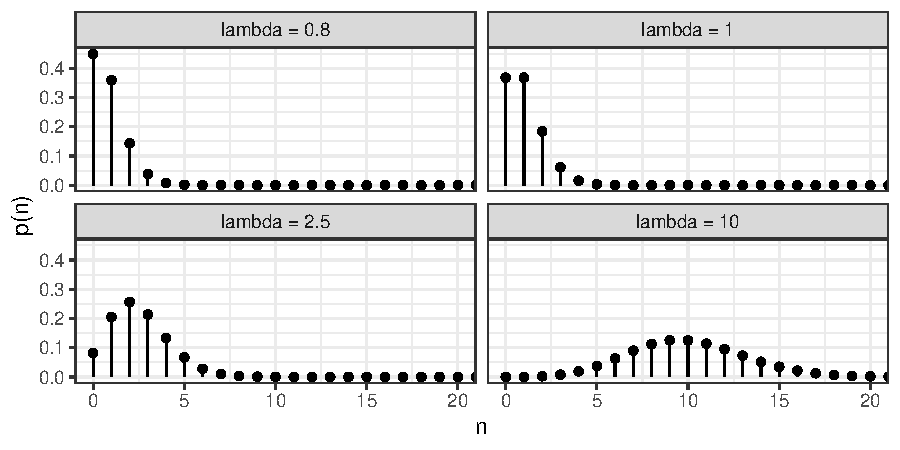
\includegraphics[width=6cm]{_bookdown_files/_main_files/figure-latex/plot-poisson-1.pdf}
      \label{fig:plot-poisson}
    \end{figure}

  \end{block}
\end{column}

\begin{column}{0.45\linewidth}
  \begin{block}{Distribuzione Gamma}
    $$
    f_Z(z) = \frac{\rho^\alpha}{\Gamma(\alpha)}z^{\alpha-1}e^{-\rho z}, \quad \alpha > 0, \ \rho > 0
    $$
    
    \begin{figure}
      \centering
      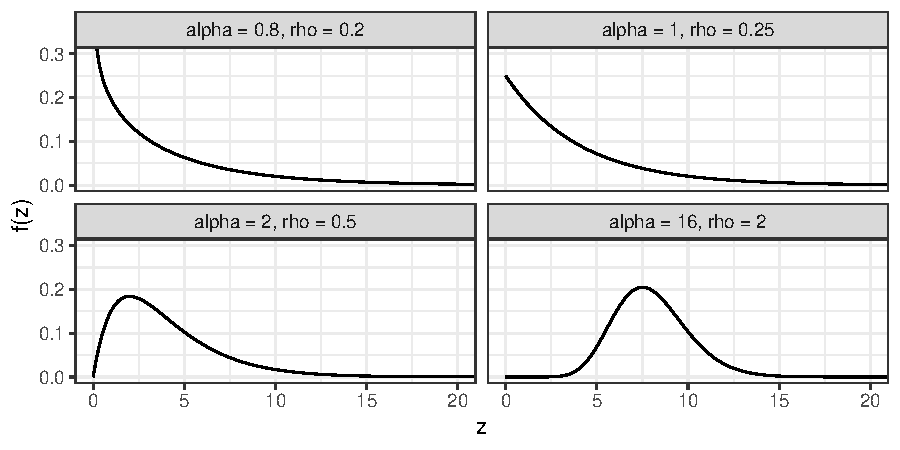
\includegraphics[width=6cm]{_bookdown_files/_main_files/figure-latex/plot-gamma-1.pdf}
      \label{fig:plot-gamma}
    \end{figure}

  \end{block}
\end{column}

\end{columns}

\end{frame}


%%%%%%%%%%%%%%%%%%%%%%%%%%%%%%%%%%%%%%%%%%%%%%%%%%%%%%%%%%%%%
\begin{frame}
\frametitle{Pricing Tecnico e Commerciale}

\fontsize{9pt}{11pt}\selectfont


% \begin{columns}[t, totalwidth=1.02\textwidth]
\begin{columns}[T]

\begin{column}{0.5\linewidth}
  \uncover<1->{
    \begin{block}{Definizione di Premio}
      \vspace{0.2cm}
      % \begin{center}
        \begin{tikzpicture}
          \node[text width=6cm, align=left] at (0, 0) (p1) {$P^{(\textrm{risk})}_i=E(S_i)$ \\ $P^{(\textrm{tech})}_i = E(S_i) + \textrm{Expenses}_i$};
          \node[text width=6cm, align=left] at (0, -3cm) (p2) {$P^{(\textrm{tariff})}_i$ \\ $P^{(\textrm{offer})}_i = P^{(\textrm{tariff})}_i - \textrm{Discount}_i$};
          \draw[black, ->] 
            (-2.5cm, -0.6cm) -- node[right, text width=8cm, align=left]{\footnotesize Altri Caricamenti \\ Vincoli Normativi \\ Commercializzazioni} (-2.5cm, -2.4cm);
        \end{tikzpicture}
      % \end{center}
    \end{block}
  }
\end{column}

\begin{column}{0.5\linewidth}
  \uncover<2->{
    \begin{block}{Ottimizzazione del Prezzo}
      
      % \vfill
      % \vspace{0.5cm}
      \vspace{0.2cm}
      
      Si basa su
      \begin{enumerate}
        \item Pricing Tecnico
        \item Aspettativa del Cliente
        \item Strategia di Business
      \end{enumerate}
    
      % \vfill
      \vspace{0.2cm}
      
      Ulteriori modelli
      \begin{itemize}
        \item New Business: Probabilità di Conversion
        \item Rinnovi: Probabilità di Retention
      \end{itemize}

    \end{block}
  }
\end{column}

\end{columns}

\end{frame}





%%%%%%%%%%%%%%%%%%%%%%%%%%%%%%%%%%%%%%%%%%%%%%%%%%%%%%%%%%%%%
\section{Modelli Statistici per il Pricing nelle Assicurazioni Danni}

%%%%%%%%%%%%%%%%%%%%%%%%%%%%%%%%%%%%%%%%%%%%%%%%%%%%%%%%%%%%%
\subsection{Modelli Lineari Generalizzati (GLM)}

\begin{frame}
\frametitle{Modelli Lineari Generalizzati (GLM)}
\fontsize{9pt}{11pt}\selectfont


\begin{block}{Modelli Lineari Generalizzati (GLM)}
  
  Dato $\mathcal{D} = \left\{ (\boldsymbol{x}_1, \omega_1, y_1), \dots,  (\boldsymbol{x}_n, \omega_n, y_n) \right\}$
  
  con $\boldsymbol{y} = (y_1, \dots, y_n)^t$ realizzazione di $\boldsymbol{Y} = (Y_1, \dots, Y_n)^t$.
  
  \vspace{0.2cm}
  Assumiamo che:
  \begin{enumerate}
    \item $\boldsymbol{Y} = (Y_1, \dots, Y_n)^t$ siano indipendenti con distribuzione appartenente a una stessa famiglia esponenziale lineare:
    $$f(y_i; \theta_i, \phi, \omega_i) = \exp{\left\{ \frac{\omega_i}{\phi} \left[y_i\theta_i - b(\theta_i) \right] \right\}} \ c(y_i, \phi, \omega_i), \quad y_i\in \mathcal{Y}\subseteq\mathbb{R}$$
    \item $\boldsymbol{x}_i = \left(1, x_{i1}, \dots, x_{ip} \right)^t$ agisca su $Y_i$ tramite il predittore lineare $\eta_i$
    $$\eta_i = \beta_0 + \beta_1 x_{i1} + \beta_2 x_{i2} + \dots + \beta_p x_{ip}$$
    \item $\eta_i$ sia legato a $\mu_i=E(Y_i)$ tramite la funzione legame $g(\cdot)$
    $$g(\mu_i) = \eta_i = \boldsymbol{x}_i^t \boldsymbol{\beta}$$
  \end{enumerate}
\end{block}

\end{frame}



%%%%%%%%%%%%%%%%%%%%%%%%%%%%%%%%%%%%%%%%%%%%%%%%%%%%%%%%%%%%%
\begin{frame}
\frametitle{Stima di un GLM}
\fontsize{9pt}{11pt}\selectfont


\begin{columns}[T]

\begin{column}{0.5\linewidth}
  \uncover<1->{
    \begin{block}{Stima di massima verosimiglianza}
      Data la funzione di verosimiglianza
      $$
      \begin{array}{cccc}
        L: & \mathbb{R}^{p+1} \times \Lambda & \longrightarrow & [0, +\infty[ \\
           & \left(\boldsymbol{\beta}, \phi\right) & \longmapsto & f_{\boldsymbol{Y}}(\boldsymbol{y};       \boldsymbol{ \theta}, \phi)
      \end{array}
      $$
  
      La stima di massima verosimiglianza è:
      $$
      \hat{\boldsymbol{\beta}} = \argmax_{\boldsymbol{\beta}\in\mathbb{R}^{p+1}}{L\left(\boldsymbol{\beta}, \phi; \boldsymbol{y}\right)}
      $$
    \end{block}
  }
\end{column}

\begin{column}{0.5\linewidth}
  \uncover<2->{
    \begin{block}{Devianza}
      La devianza è
      $$
      D(\hat{\boldsymbol{\beta}}, \boldsymbol{y}) =
        -2\phi\left(
        \ell\left(\hat{\boldsymbol{\beta}}, \phi; \boldsymbol{y}\right)
        - \ell_{S}\left(\boldsymbol{\beta}^*, \phi; \boldsymbol{y}\right)
        \right)
      $$
      dove $\ell\left(\hat{\boldsymbol{\beta}}, \phi; \boldsymbol{y}\right) = \log{L\left(\hat{\boldsymbol{\beta}}, \phi; \boldsymbol{y}\right)}$ \newline e $\boldsymbol{\beta}^*$ sono i parametri del modello saturo.
    
      \vspace{0.2cm}
      
      La stima di massima verosimiglianza può essere ottenuta come:
      $$
      \hat{\boldsymbol{\beta}} = \argmin_{\boldsymbol{\beta}\in\mathbb{R}^{p+1}}{D(\boldsymbol{\beta}, \boldsymbol{y})}
      $$
    \end{block}
  }

\end{column}

\end{columns}


\end{frame}



%%%%%%%%%%%%%%%%%%%%%%%%%%%%%%%%%%%%%%%%%%%%%%%%%%%%%%%%%%%%%
\begin{frame}
\frametitle{Effetto delle variabili in un GLM}
\fontsize{9pt}{11pt}\selectfont

\begin{figure}
  \centering
  \begin{subfigure}[b]{4.8cm}
    \centering
    \caption{Quantitativa}
    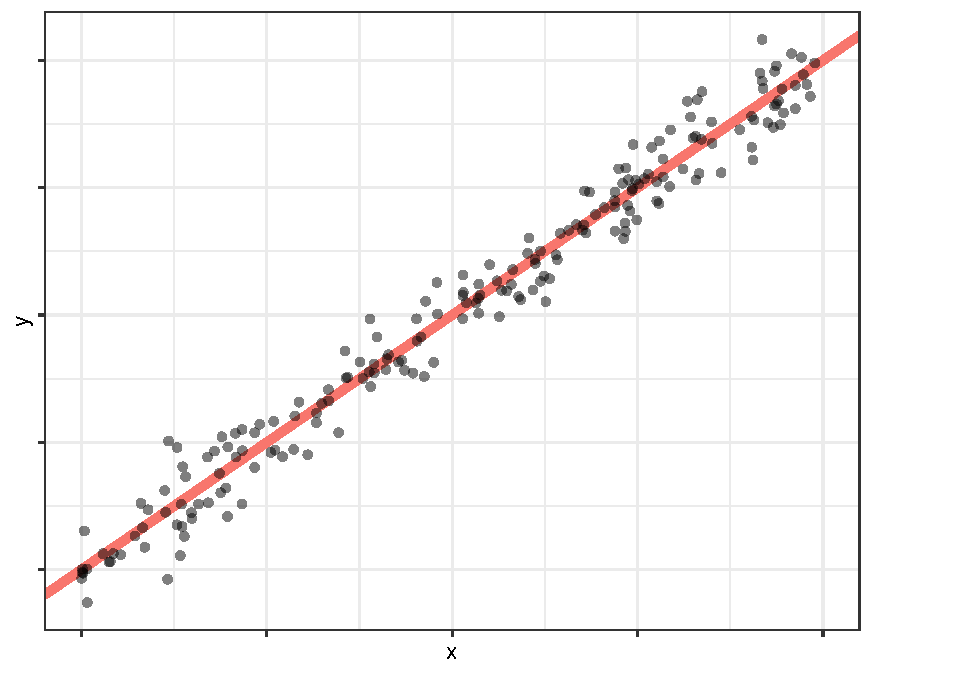
\includegraphics[width=4cm]{_bookdown_files/_main_files/figure-latex/expl-var-types-1.pdf}
  \end{subfigure}
  \qquad
  \begin{subfigure}[b]{4.8cm}
    \centering
    \caption{Qualitativa}
    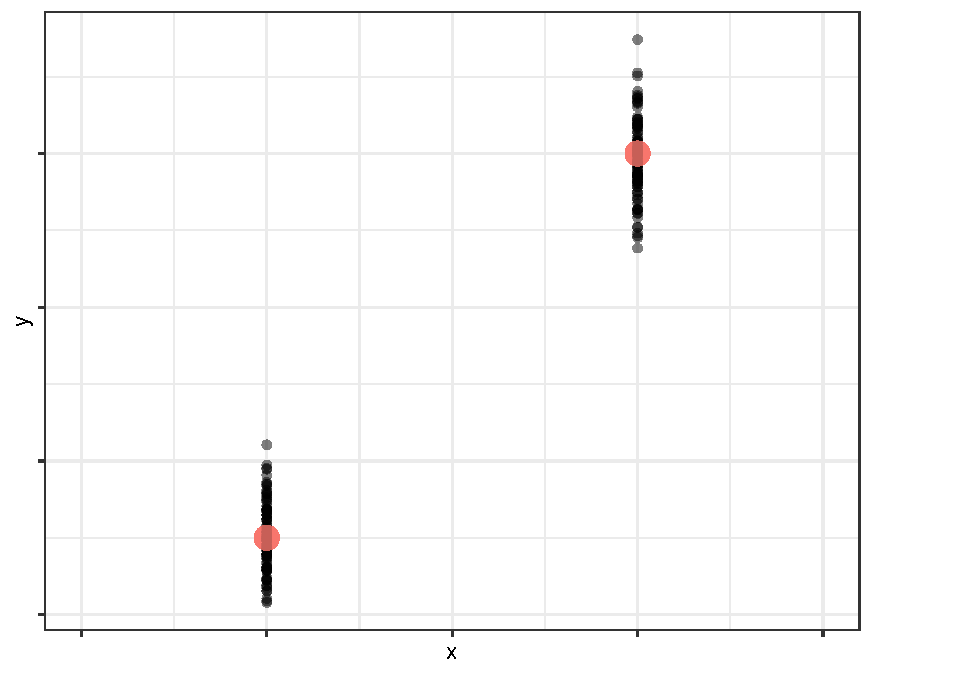
\includegraphics[width=4cm]{_bookdown_files/_main_files/figure-latex/expl-var-types-2.pdf}
  \end{subfigure}
  \par\medskip
  \begin{subfigure}[b]{4.8cm}
  % \begin{subfigure}[b]{5.9cm}
    \centering
    \caption{Quantitativa e qualitativa \\ senza interazione}
    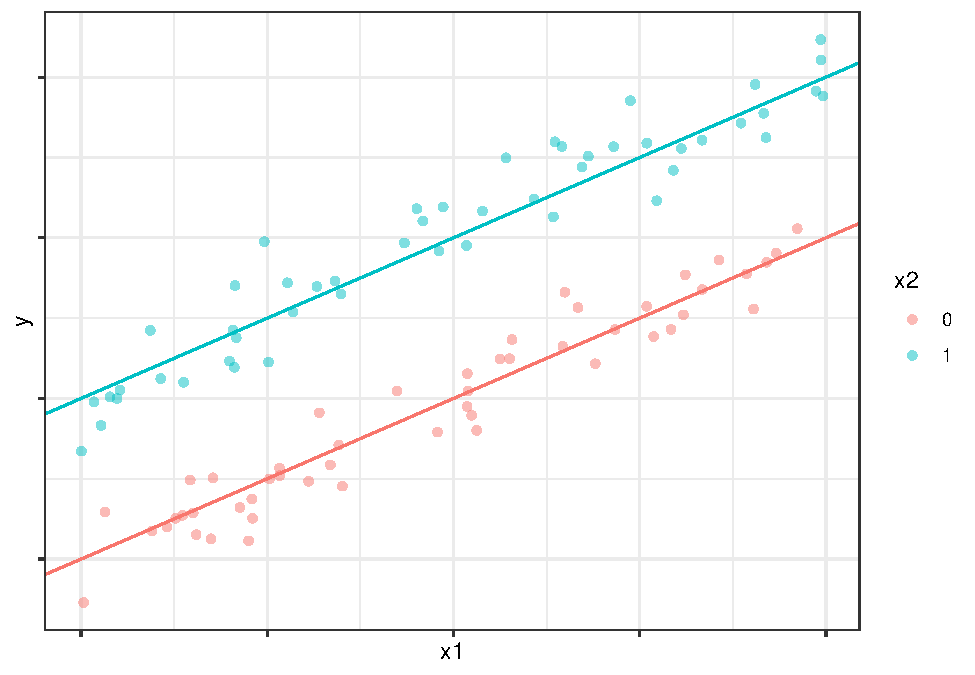
\includegraphics[width=4cm]{_bookdown_files/_main_files/figure-latex/expl-var-types-3.pdf}
  \end{subfigure}
  \qquad
  \begin{subfigure}[b]{4.8cm}
  % \begin{subfigure}[b]{5.9cm}
    \centering
    \caption{Quantitativa e qualitativa \\ con interazione}
    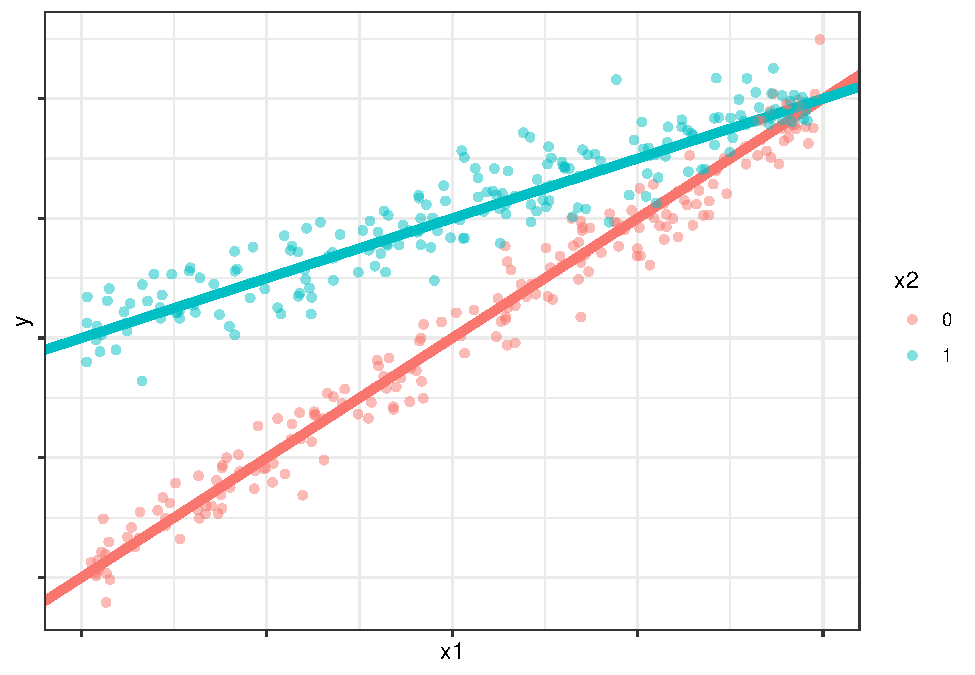
\includegraphics[width=4cm]{_bookdown_files/_main_files/figure-latex/expl-var-types-4.pdf}
  \end{subfigure}
\end{figure}

\end{frame}




%%%%%%%%%%%%%%%%%%%%%%%%%%%%%%%%%%%%%%%%%%%%%%%%%%%%%%%%%%%%%
\begin{frame}
\frametitle{Variabili quantitative ed effetti non lineari}

\fontsize{9pt}{11pt}\selectfont

\begin{figure}
  \centering
  \begin{subfigure}[b]{4.8cm}
    \centering
    \caption{Polinomiale di grado 2}
    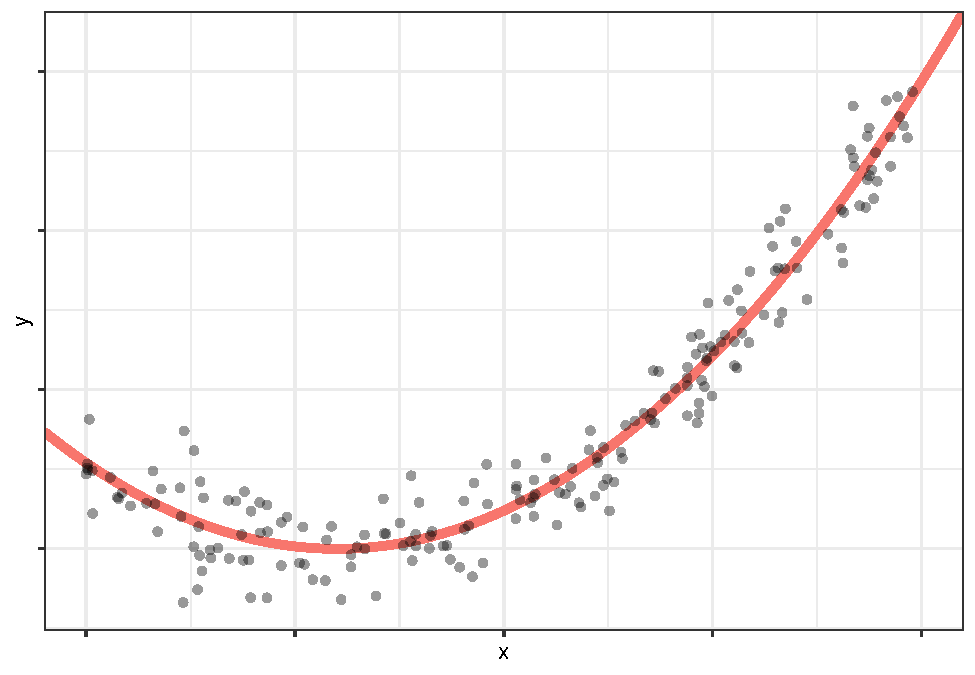
\includegraphics[width=4cm]{_bookdown_files/_main_files/figure-latex/expl-var-quant-effect-1.pdf}
  \end{subfigure}
  \qquad
  \begin{subfigure}[b]{4.8cm}
    \centering
    \caption{Polinomiale di grado 4}
    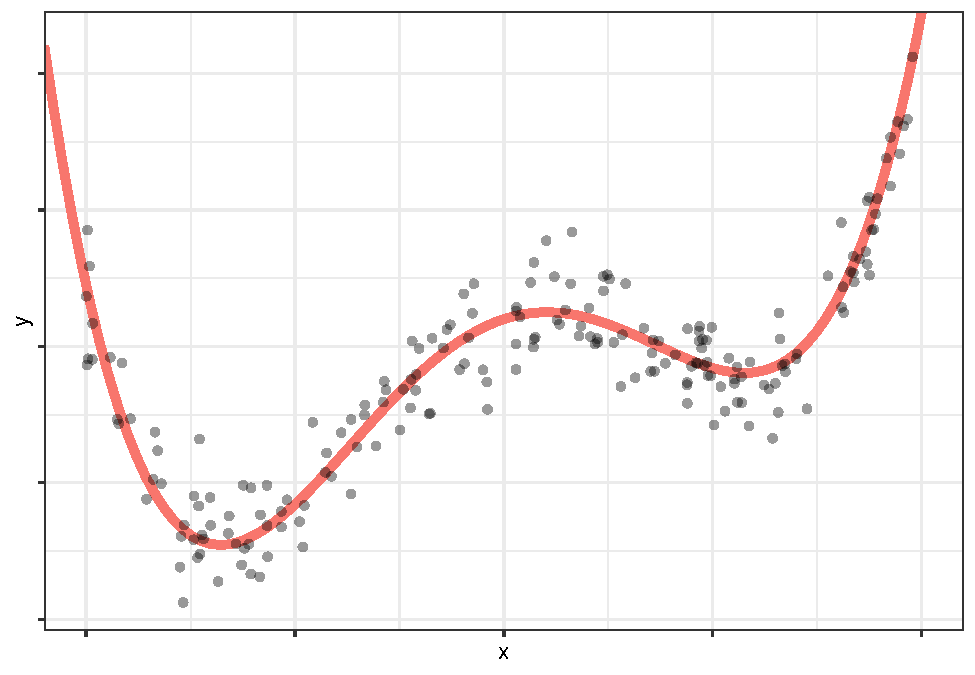
\includegraphics[width=4cm]{_bookdown_files/_main_files/figure-latex/expl-var-quant-effect-2.pdf}
  \end{subfigure}
  \par\medskip
  \begin{subfigure}[b]{4.8cm}
    \centering
    \caption{Piece-wise lineare}
    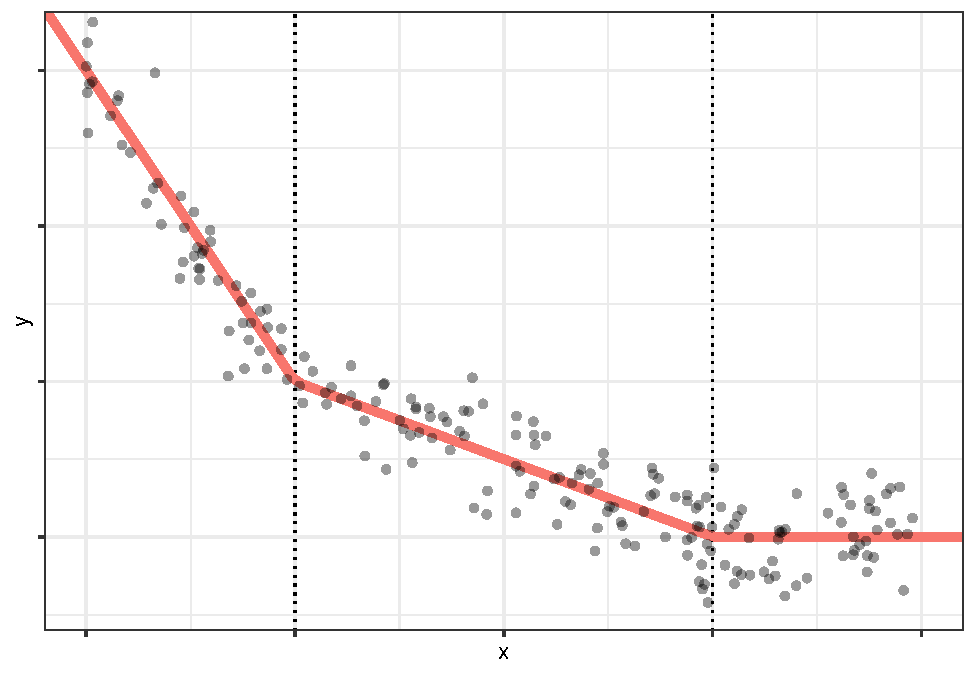
\includegraphics[width=4cm]{_bookdown_files/_main_files/figure-latex/expl-var-quant-effect-3.pdf}
  \end{subfigure}
  \qquad
  \begin{subfigure}[b]{4.8cm}
    \centering
    \caption{Piece-wise polinomiale di grado 2}
    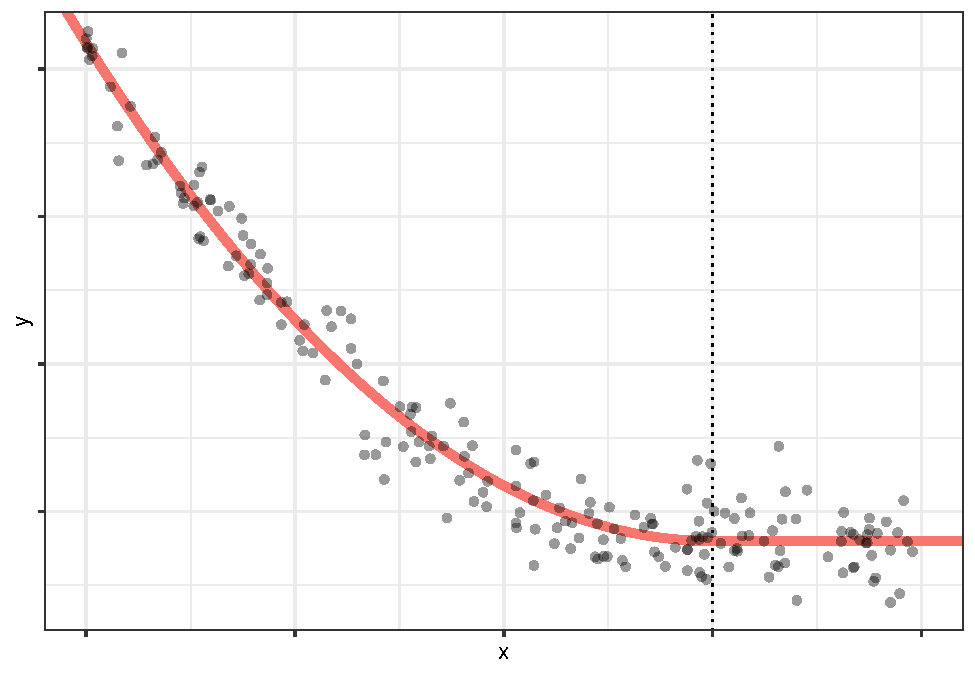
\includegraphics[width=4cm]{_bookdown_files/_main_files/figure-latex/expl-var-quant-effect-4.pdf}
  \end{subfigure}
\end{figure}

\end{frame}



%%%%%%%%%%%%%%%%%%%%%%%%%%%%%%%%%%%%%%%%%%%%%%%%%%%%%%%%%%%%%
\begin{frame}
\frametitle{Funzione Legame e risposta}

\fontsize{9pt}{11pt}\selectfont

\begin{figure}
  \centering
  \begin{subfigure}[b]{4.8cm}
    \centering
    \caption{Normale - identità}
    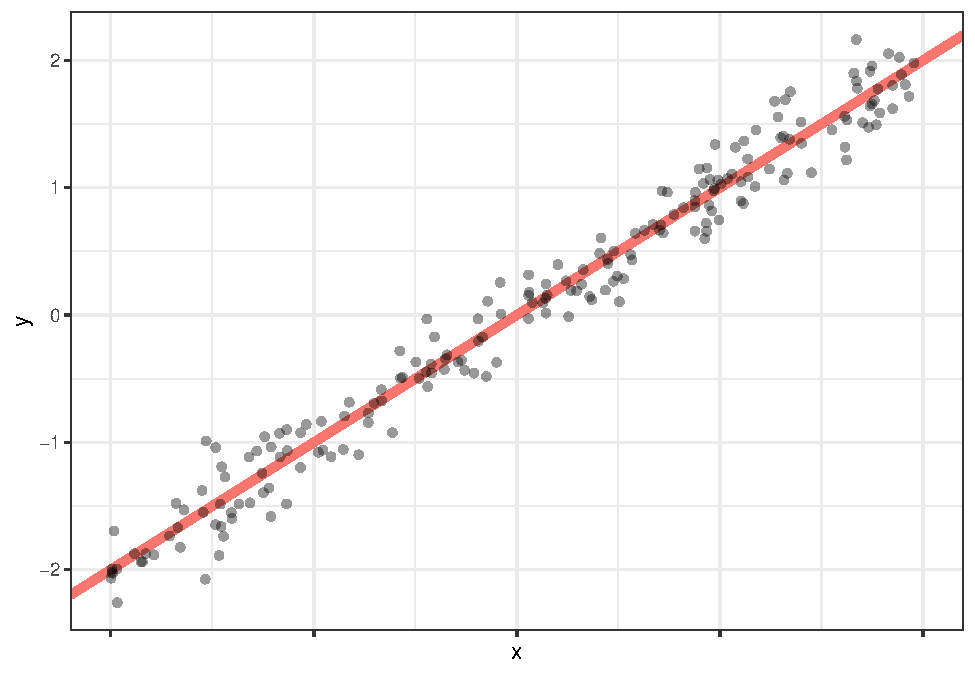
\includegraphics[width=4cm]{_bookdown_files/_main_files/figure-latex/resp-var-1.pdf}
  \end{subfigure}
  \qquad
  \begin{subfigure}[b]{4.8cm}
    \centering
    \caption{Binomiale - logit}
    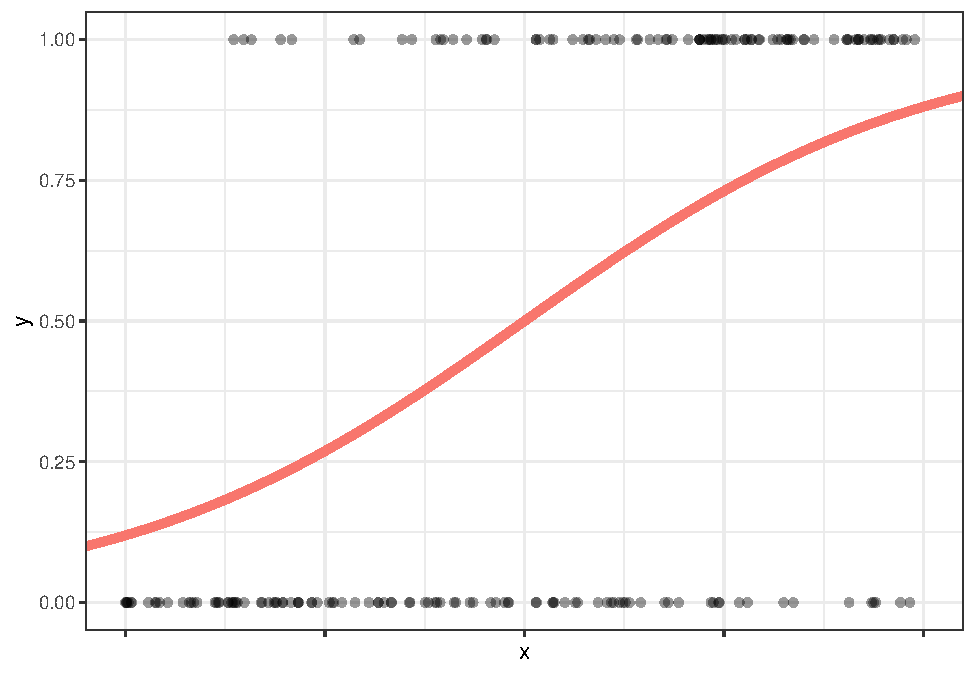
\includegraphics[width=4cm]{_bookdown_files/_main_files/figure-latex/resp-var-2.pdf}
  \end{subfigure}
  \par\medskip
  \begin{subfigure}[b]{4.8cm}
    \centering
    \caption{Poisson - log}
    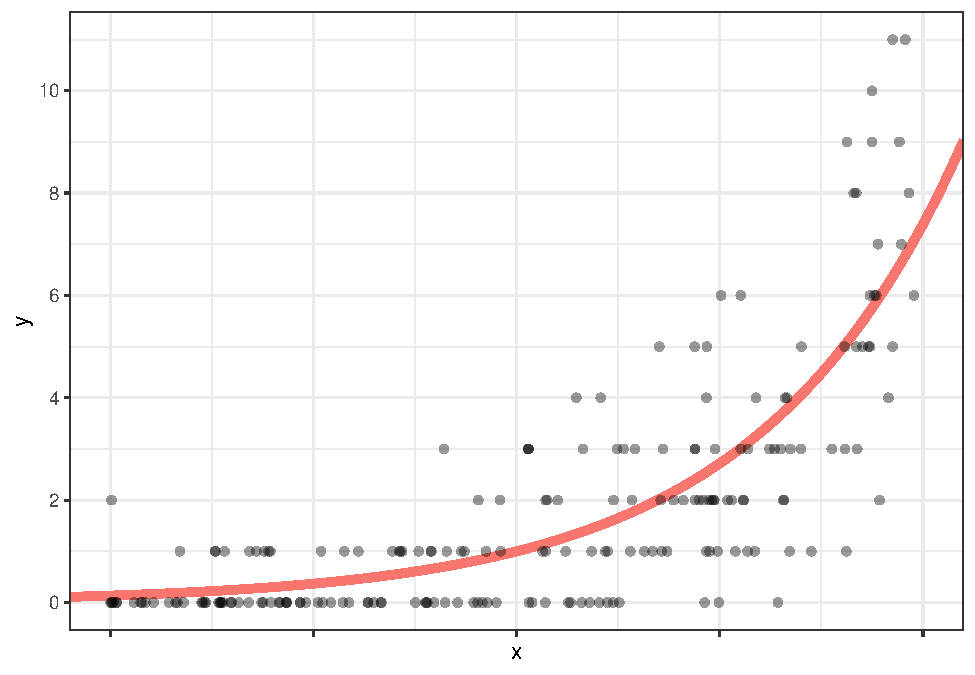
\includegraphics[width=4cm]{_bookdown_files/_main_files/figure-latex/resp-var-3.pdf}
  \end{subfigure}
  \qquad
  \begin{subfigure}[b]{4.8cm}
    \centering
    \caption{Gamma - log}
    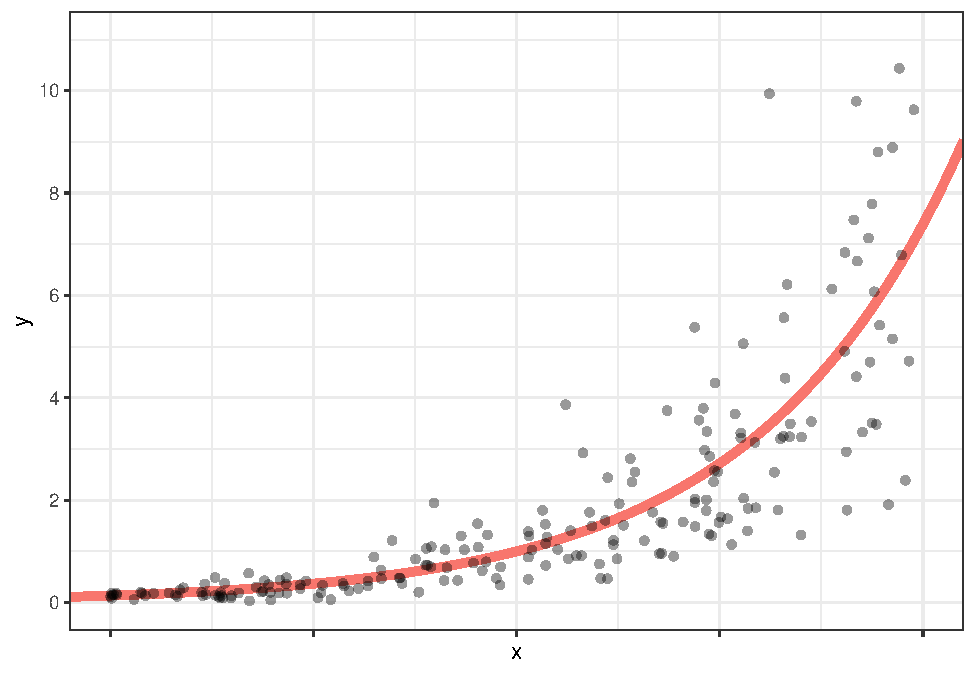
\includegraphics[width=4cm]{_bookdown_files/_main_files/figure-latex/resp-var-4.pdf}
  \end{subfigure}
\end{figure}

\end{frame}



%%%%%%%%%%%%%%%%%%%%%%%%%%%%%%%%%%%%%%%%%%%%%%%%%%%%%%%%%%%%%
\begin{frame}
\frametitle{Grafici per visualizzare l'effetto delle variabili}

\fontsize{9pt}{11pt}\selectfont

\begin{figure}
  \centering
  \begin{subfigure}[b]{4.8cm}
    \centering
    % \caption{No effect - ungrouped}
    \caption{Nessun effetto - non raggruppati}
    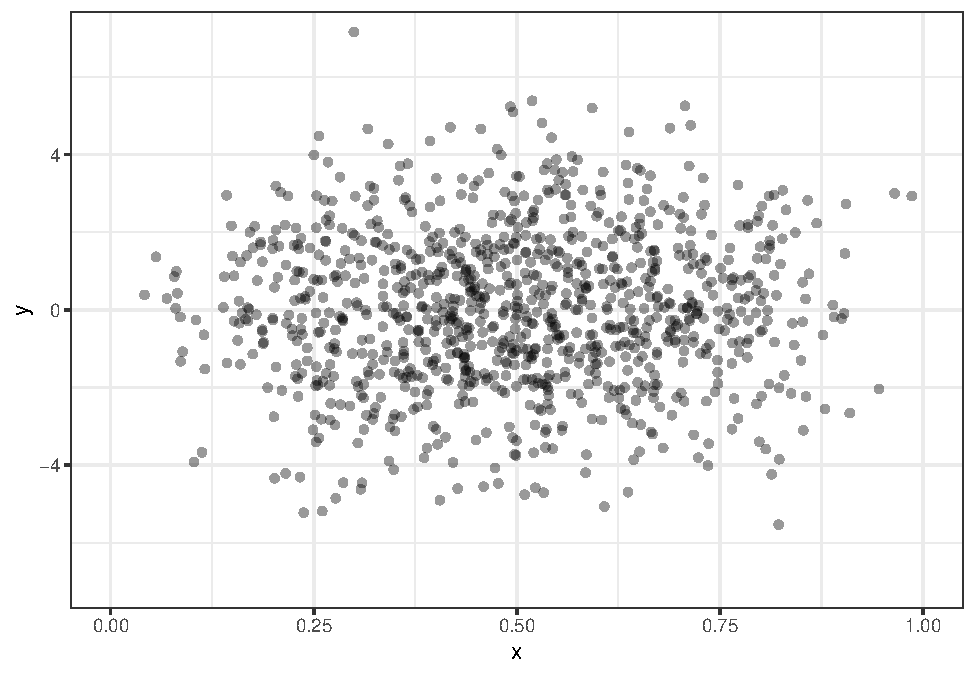
\includegraphics[width=4cm]{_bookdown_files/_main_files/figure-latex/var-selection-1.pdf}
  \end{subfigure}
  \qquad
  \begin{subfigure}[b]{4.8cm}
    \centering
    % \caption{Positive effect - ungrouped}
    \caption{Effetto positivo - non raggruppati}
    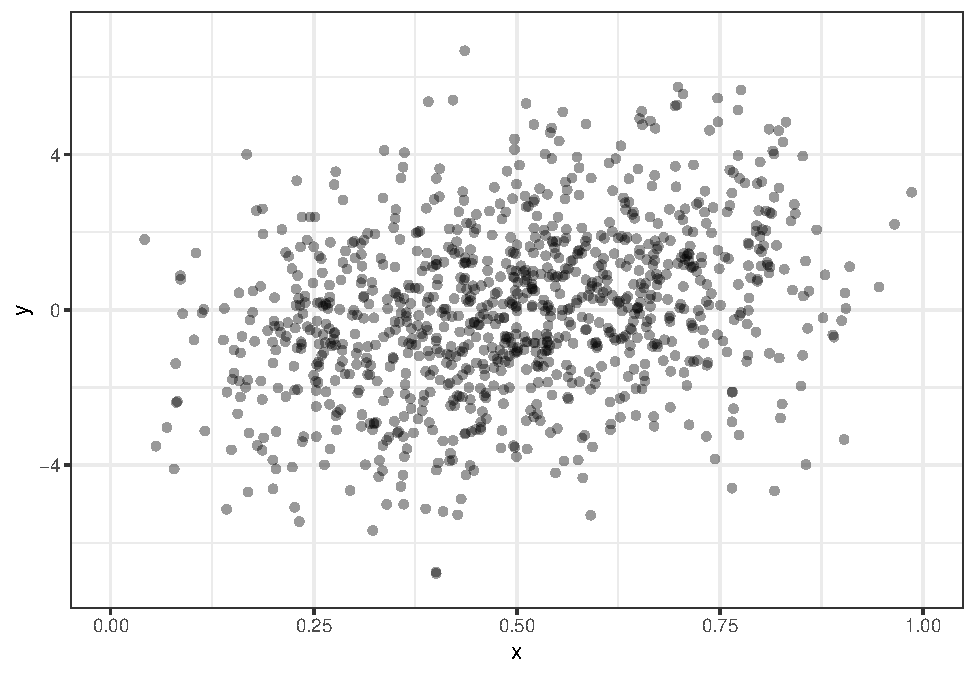
\includegraphics[width=4cm]{_bookdown_files/_main_files/figure-latex/var-selection-2.pdf}
  \end{subfigure}
  \par\medskip
  \begin{subfigure}[b]{4.8cm}
    \centering
    % \caption{No effect - grouped}
    \caption{Nessun effetto - raggruppati}
    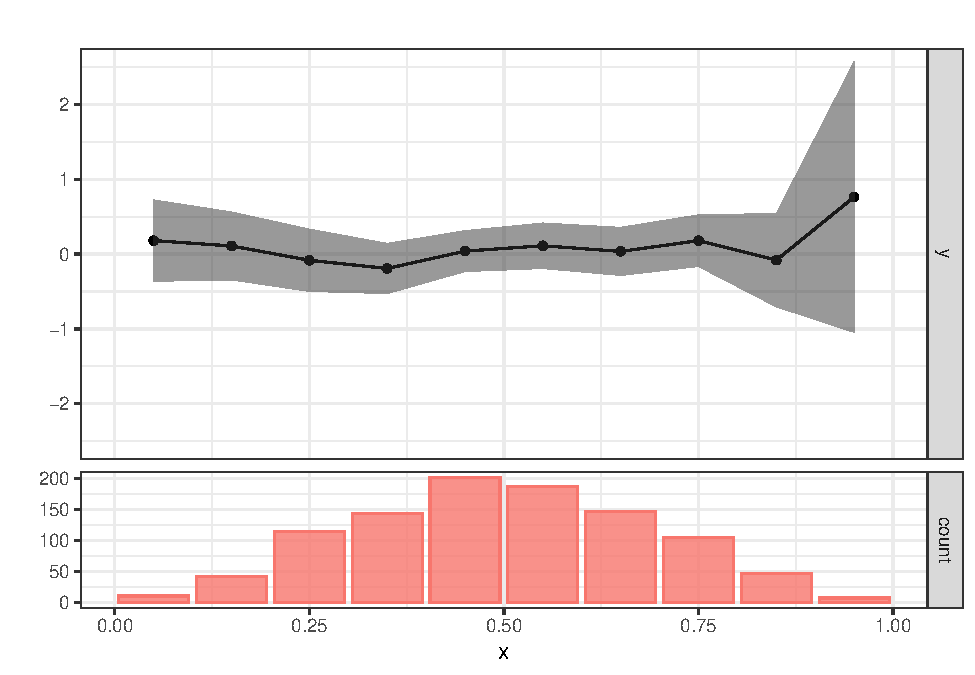
\includegraphics[width=4cm]{_bookdown_files/_main_files/figure-latex/var-selection-3.pdf}
  \end{subfigure}
  \qquad
  \begin{subfigure}[b]{4.8cm}
    \centering
    % \caption{Positive effect - grouped}
    \caption{Effetto positivo - raggruppati}
    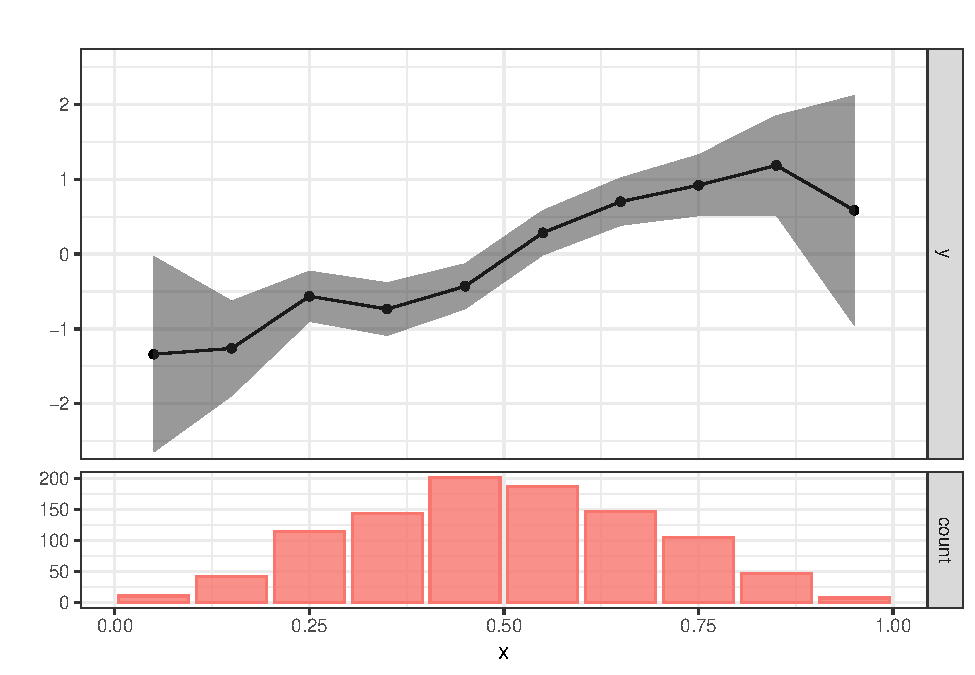
\includegraphics[width=4cm]{_bookdown_files/_main_files/figure-latex/var-selection-4.pdf}
  \end{subfigure}
\end{figure}

\end{frame}




%%%%%%%%%%%%%%%%%%%%%%%%%%%%%%%%%%%%%%%%%%%%%%%%%%%%%%%%%%%%%
\begin{frame}
\frametitle{Criteri per la selezione delle variabili nei GLM}

\fontsize{9pt}{11pt}\selectfont

\begin{block}{Criteri per la selezione delle variabili}
  \begin{itemize}
    \item Visualizzazione
    \item Test di verifica di ipotesi
    $$
    \begin{cases}
      H_0: & \beta_{j_k} = 0 \ \forall k \in \{1, 2, \dots, s\} \\
      H_1: & \exists k: \beta_{j_k} \neq 0
    \end{cases}
    $$
    \item Criteri di informazione
    \begin{align*}
      AIC & = -2\ell(\boldsymbol{\beta}) + 2 (p+1) \\
      BIC & = -2\ell(\boldsymbol{\beta}) + \log(n) (p+1)
    \end{align*}
    \item Divisione del dataset tra training set e test set
    \item Cross validation
  \end{itemize}
  \vspace{0.2cm}
  \hspace{2cm}
  $\Longrightarrow$ Algoritmi stepwise
\end{block}


\end{frame}


%%%%%%%%%%%%%%%%%%%%%%%%%%%%%%%%%%%%%%%%%%%%%%%%%%%%%%%%%%%%%
\subsection{Modelli Additivi Generalizzati (GAM)}


%%%%%%%%%%%%%%%%%%%%%%%%%%%%%%%%%%%%%%%%%%%%%%%%%%%%%%%%%%%%%
\begin{frame}
\frametitle{Modelli Additivi Generalizzati (GAM)}

\fontsize{9pt}{11pt}\selectfont

\begin{columns}[T]
\begin{column}{0.5\linewidth}
  \begin{block}{Modello Additivo Generalizzato (GAM)}
    \begin{enumerate}
      \item Variabile risposta $\boldsymbol{Y}$ come GLM;
      \item Predittore lineare
      $$
      \eta_i = \boldsymbol{x}_i^t \boldsymbol{\beta} + \sum_{l=1}^{q}{f_l(z_{i,l})}, \quad i\in\{1,2,\dots,n\}
      $$
      con $f_l(\cdot)$ spline cubica;
      \item Funzione legame $g(\cdot)$ come GLM.
    \end{enumerate}
  \end{block}
\end{column}

\begin{column}{0.5\linewidth}
  \begin{block}{Stima di Massima Verosimiglianza con Penalizzazione}
    $$
    \boldsymbol{\hat{f}} = \argmin_{\boldsymbol{f}}
    {\left\{
      D(\boldsymbol{f}, \boldsymbol{y})
        + \sum_{l=1}^{q}{
          \lambda_l \int_{a_l}^{b_l}{\left( f_l''(x_l) \right)^2 dx}
        }
    \right\}
    }
    $$
    con $\lambda_1, \lambda_2, \dots, \lambda_q$ iperparametri di smoothing.
  \end{block}
\end{column}

\end{columns}

\end{frame}


%%%%%%%%%%%%%%%%%%%%%%%%%%%%%%%%%%%%%%%%%%%%%%%%%%%%%%%%%%%%%
\begin{frame}
\frametitle{GAM: esempio}

\fontsize{9pt}{11pt}\selectfont

\begin{figure}
  \centering
  \begin{subfigure}[b]{4.8cm}
    \centering
    \caption{$\lambda = 0$}
    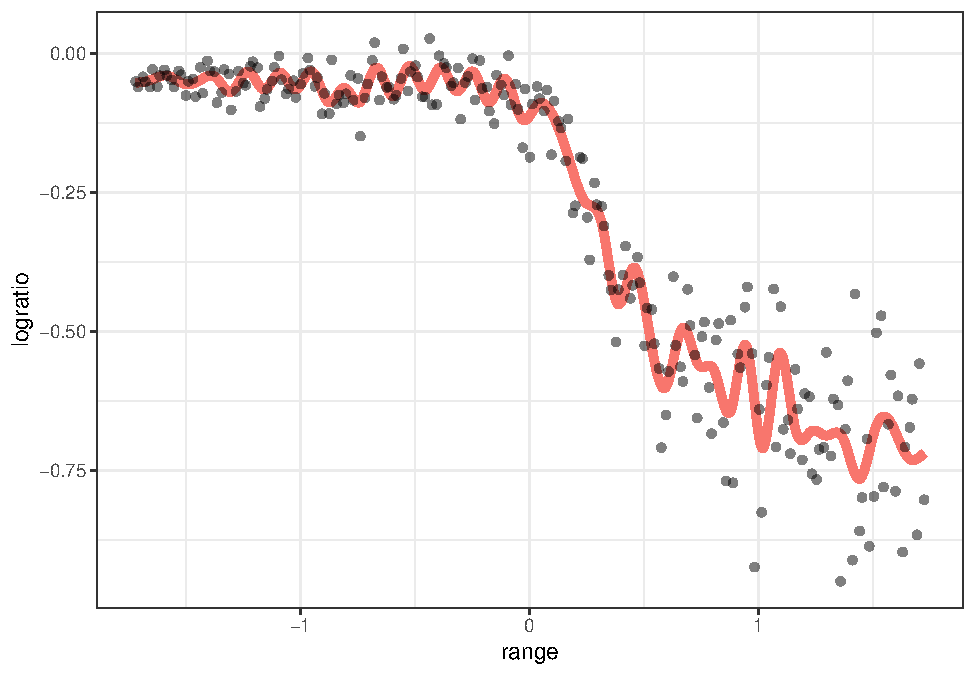
\includegraphics[width=4cm]{_bookdown_files/_main_files/figure-latex/gam-lambda-1.pdf}
  \end{subfigure}
  \qquad
  \begin{subfigure}[b]{4.8cm}
    \centering
    \caption{$\lambda = 10$}
    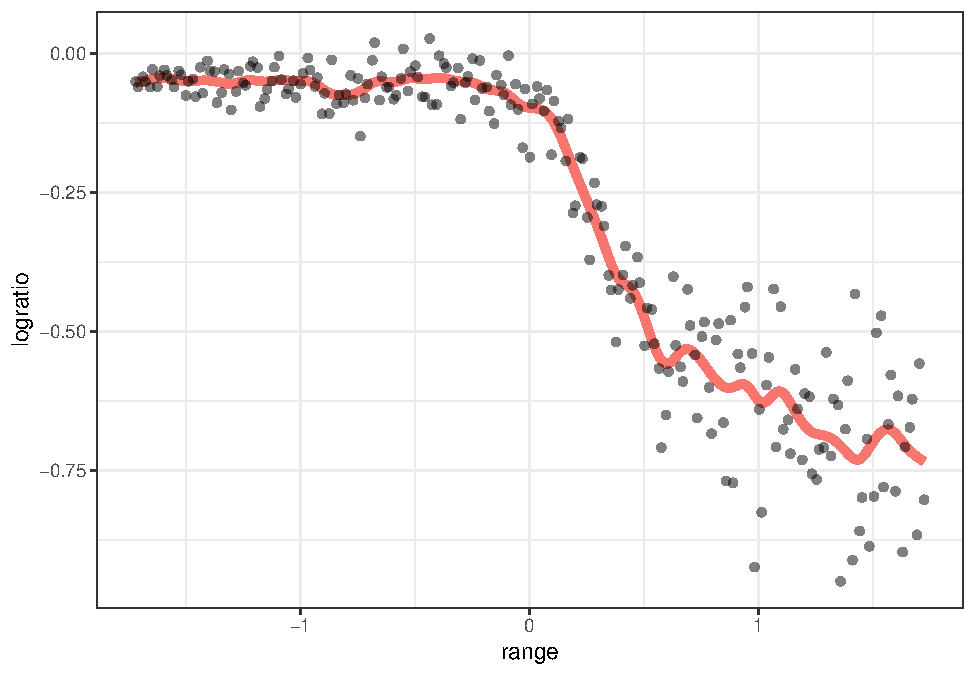
\includegraphics[width=4cm]{_bookdown_files/_main_files/figure-latex/gam-lambda-2.pdf}
  \end{subfigure}
  \par\medskip
  \begin{subfigure}[b]{4.8cm}
    \centering
    \caption{$\lambda = 10^3$}
    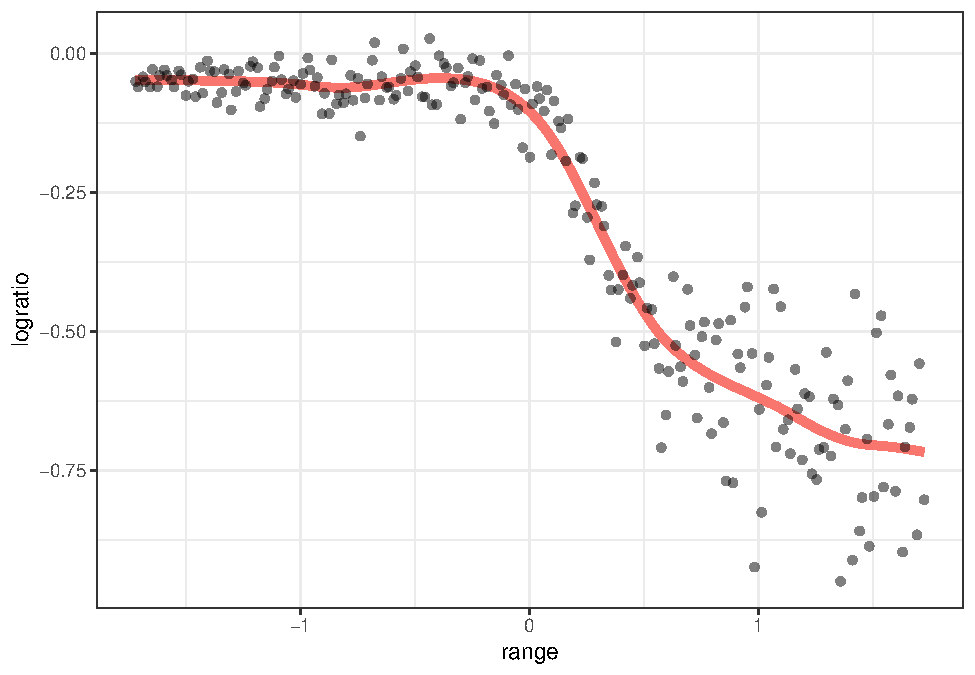
\includegraphics[width=4cm]{_bookdown_files/_main_files/figure-latex/gam-lambda-3.pdf}
  \end{subfigure}
  \qquad
  \begin{subfigure}[b]{4.8cm}
    \centering
    \caption{$\lambda = 10^6$}
    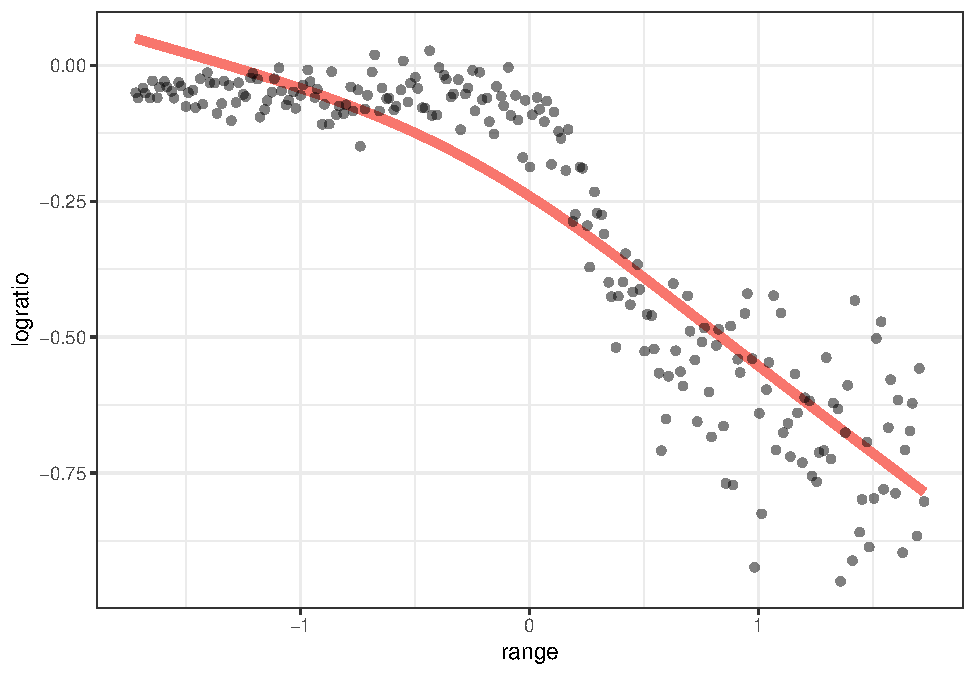
\includegraphics[width=4cm]{_bookdown_files/_main_files/figure-latex/gam-lambda-4.pdf}
  \end{subfigure}
\end{figure}

\end{frame}


%%%%%%%%%%%%%%%%%%%%%%%%%%%%%%%%%%%%%%%%%%%%%%%%%%%%%%%%%%%%%
\subsection{Stimatori Shrinkage per i GLM}

%%%%%%%%%%%%%%%%%%%%%%%%%%%%%%%%%%%%%%%%%%%%%%%%%%%%%%%%%%%%%
\begin{frame}
\frametitle{Trade-off tra Bias e Varianza}

\fontsize{9pt}{11pt}\selectfont

\begin{columns}
\begin{column}{0.8\linewidth}
  \begin{block}{Scomposizione dello scarto quadratico medio (MSE)}
    $$
    MSE\left(\tilde{\beta}_j\right) \eqdef E\left(\left(\tilde{\beta}_j - \beta_j\right)^2\right) =
    \underbrace{\left( E(\tilde{\beta}_j)-\beta_j \right)^2}_{\text{Bias}^2} +
    \underbrace{Var\left( \tilde{\beta}_j \right)}_{\text{Variance}}
    $$
    \begin{figure}
      \centering
      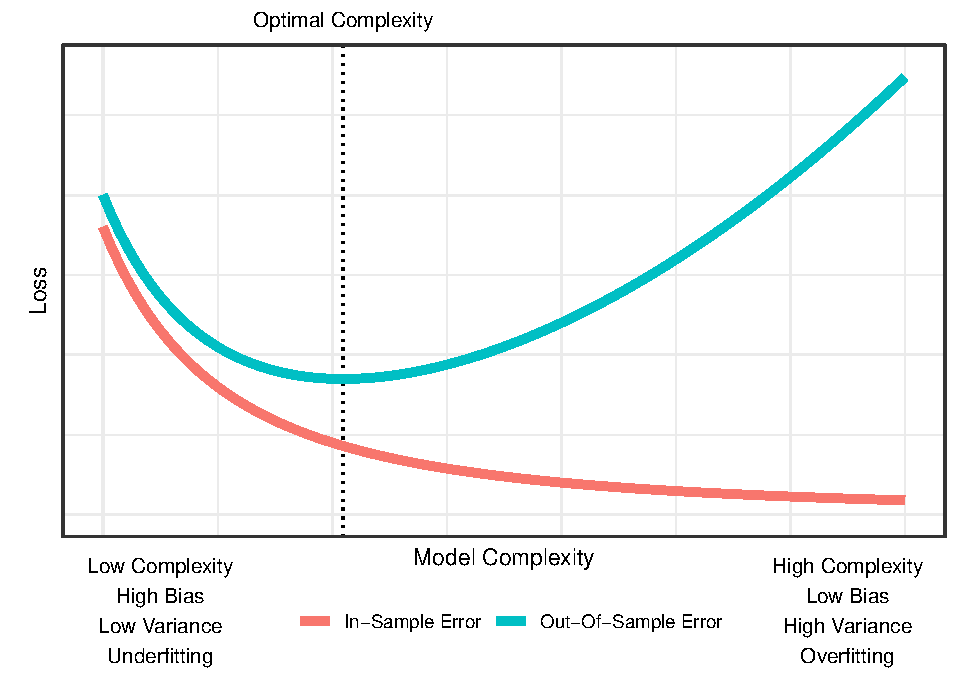
\includegraphics[width=6.5cm]{_bookdown_files/_main_files/figure-latex/bias-variance-1.pdf}
    \end{figure}
  \end{block}
\end{column}
\end{columns}

\end{frame}


%%%%%%%%%%%%%%%%%%%%%%%%%%%%%%%%%%%%%%%%%%%%%%%%%%%%%%%%%%%%%
\begin{frame}
\frametitle{Regressione Ridge}

\fontsize{9pt}{11pt}\selectfont

\begin{columns}
\begin{column}{0.8\linewidth}
  \begin{block}{Stima di Massima Verosimiglianza con Penalizzazione}
    $$
    \hat{\boldsymbol{\beta}} = \argmin_{\boldsymbol{\beta}\in\mathbb{R}^{p+1}}{\left\{D(\boldsymbol{\beta}, \boldsymbol{y}) + \lambda \|\boldsymbol{\beta}_{\setminus0}\|_2^2\right\}}
    $$
    dove
    \begin{itemize}
      \item $\|\boldsymbol{\beta}_{\setminus0}\|_2^2 = \sum_{j=1}^p{\beta_j^2}$
      \item $\lambda\ge0$ iperparametro di penalizzazione
    \end{itemize}
    
    \vspace{0.2cm}
    
    Modello sottostante:GLM
  \end{block}
\end{column}
\end{columns}

\end{frame}


%%%%%%%%%%%%%%%%%%%%%%%%%%%%%%%%%%%%%%%%%%%%%%%%%%%%%%%%%%%%%
\begin{frame}
\frametitle{Regressione Ridge: esempio}

\fontsize{9pt}{11pt}\selectfont

\begin{columns}[c]
\begin{column}{0.55\linewidth}
  \begin{figure}
    \centering
    \begin{subfigure}[b]{3cm}
      \centering
      \caption{$\lambda = 0$}
      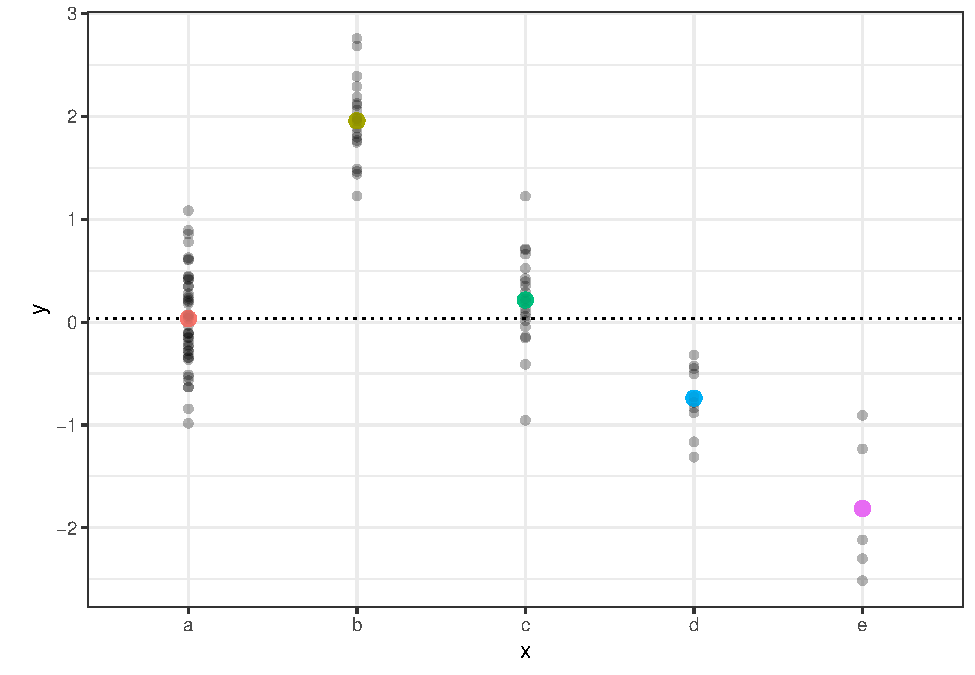
\includegraphics[width=3.5cm]{_bookdown_files/_main_files/figure-latex/ridge-lambda-1.pdf}
    \end{subfigure}
    \qquad
    \begin{subfigure}[b]{3cm}
      \centering
      \caption{$\lambda = 0.1$}
      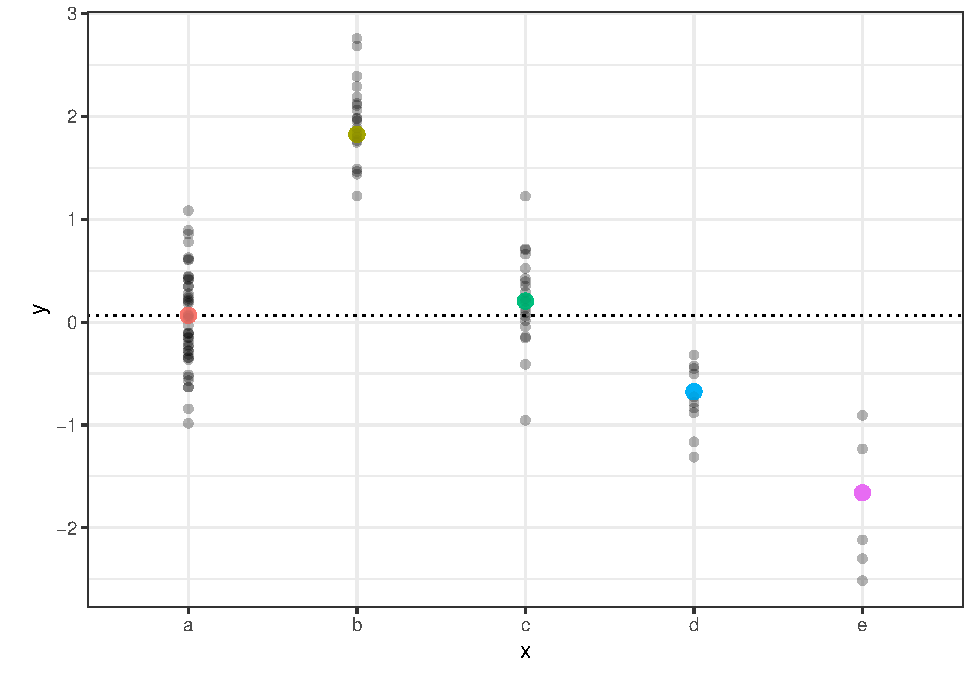
\includegraphics[width=3.5cm]{_bookdown_files/_main_files/figure-latex/ridge-lambda-2.pdf}
    \end{subfigure}
    \par\medskip
    \begin{subfigure}[b]{3cm}
      \centering
      \caption{$\lambda = 1$}
      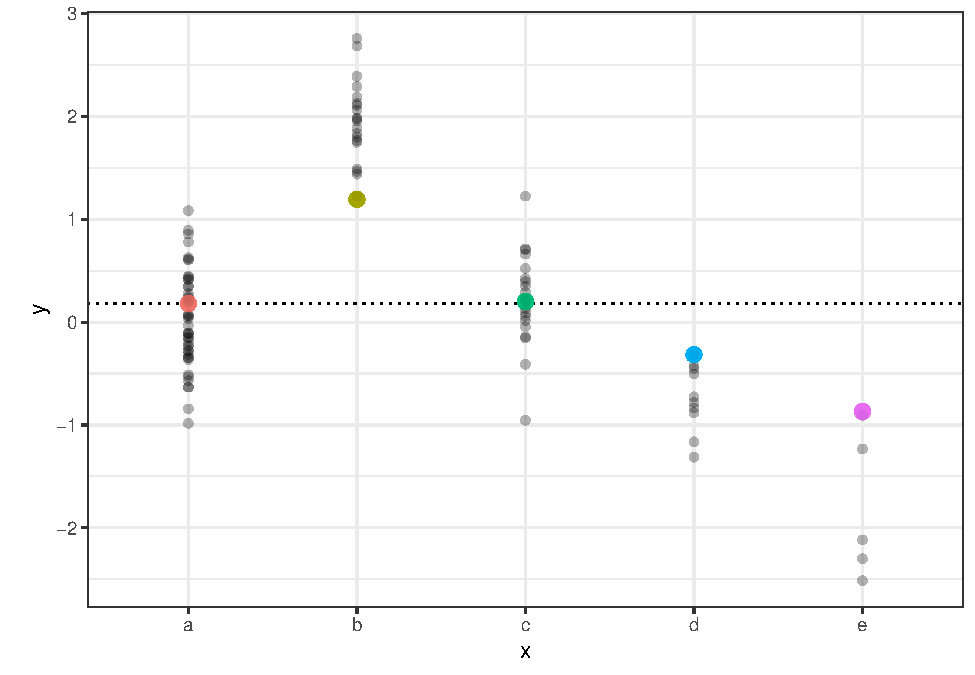
\includegraphics[width=3.5cm]{_bookdown_files/_main_files/figure-latex/ridge-lambda-3.pdf}
    \end{subfigure}
    \qquad
    \begin{subfigure}[b]{3cm}
      \centering
      \caption{$\lambda = 10$}
      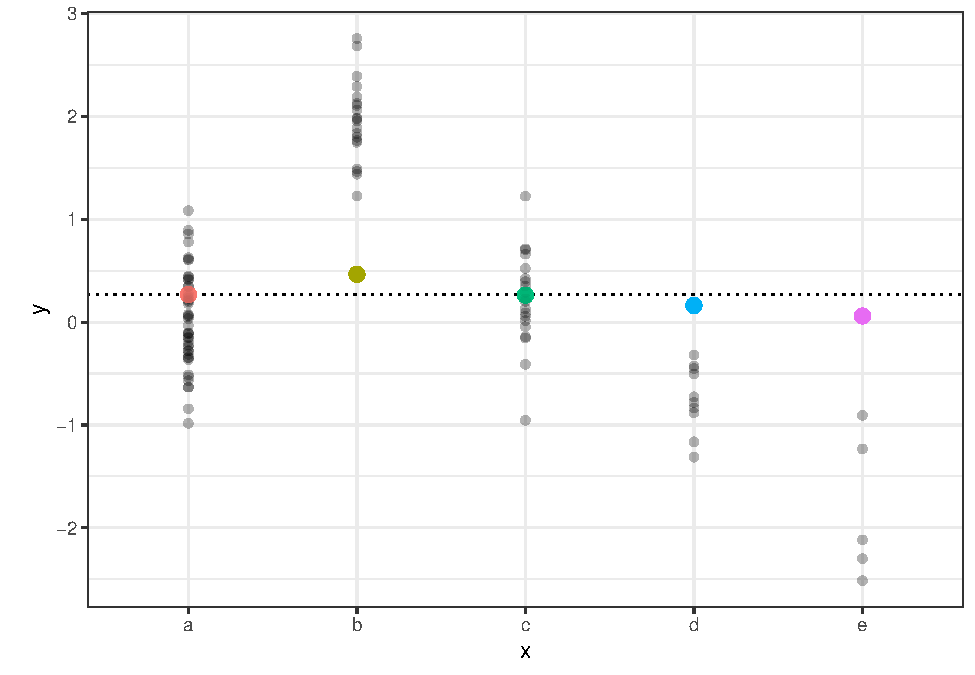
\includegraphics[width=3.5cm]{_bookdown_files/_main_files/figure-latex/ridge-lambda-4.pdf}
    \end{subfigure}
  \end{figure}
\end{column}
\begin{column}{0.45\linewidth}
  \begin{figure}
    \centering
    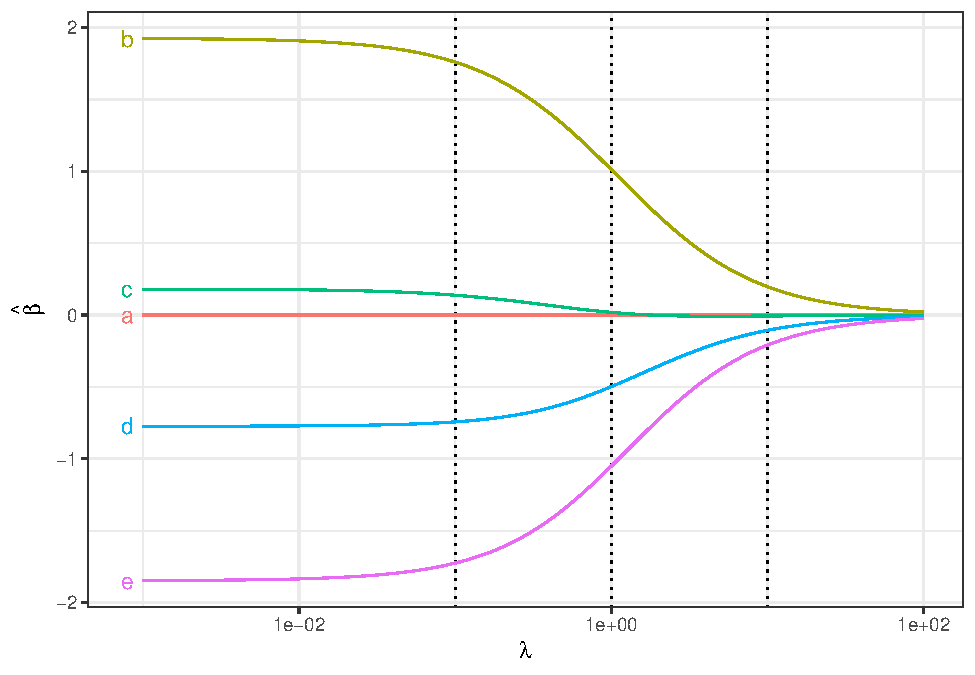
\includegraphics[width=5cm]{_bookdown_files/_main_files/figure-latex/ridge-lambda-5.pdf}
  \end{figure}
\end{column}
\end{columns}

\end{frame}


%%%%%%%%%%%%%%%%%%%%%%%%%%%%%%%%%%%%%%%%%%%%%%%%%%%%%%%%%%%%%
\begin{frame}
\frametitle{Regressione LASSO}

\fontsize{9pt}{11pt}\selectfont

\begin{columns}
\begin{column}{0.8\linewidth}
  \begin{block}{Stima di Massima Verosimiglianza con Penalizzazione}
    $$
    \hat{\boldsymbol{\beta}} = \argmin_{\boldsymbol{\beta}\in\mathbb{R}^{p+1}}{\left\{D(\boldsymbol{\beta}, \boldsymbol{y}) + \lambda \|\boldsymbol{\beta}_{\setminus0}\|_1\right\}}
    $$
    dove
    \begin{itemize}
      \item $\|\boldsymbol{\beta}_{\setminus0}\|_1 = \sum_{j=1}^p{|\beta_j|}$
      \item $\lambda\ge0$ iperparametro di penalizzazione
    \end{itemize}
    
    \vspace{0.2cm}
    
    Modello sottostante:GLM
  \end{block}
\end{column}
\end{columns}

\end{frame}

%%%%%%%%%%%%%%%%%%%%%%%%%%%%%%%%%%%%%%%%%%%%%%%%%%%%%%%%%%%%%
\begin{frame}
\frametitle{Regressione LASSO: esempio}

\fontsize{9pt}{11pt}\selectfont

\begin{columns}[c]
\begin{column}{0.55\linewidth}
  \begin{figure}
    \centering
    \begin{subfigure}[b]{3cm}
      \centering
      \caption{$\lambda = 0$}
      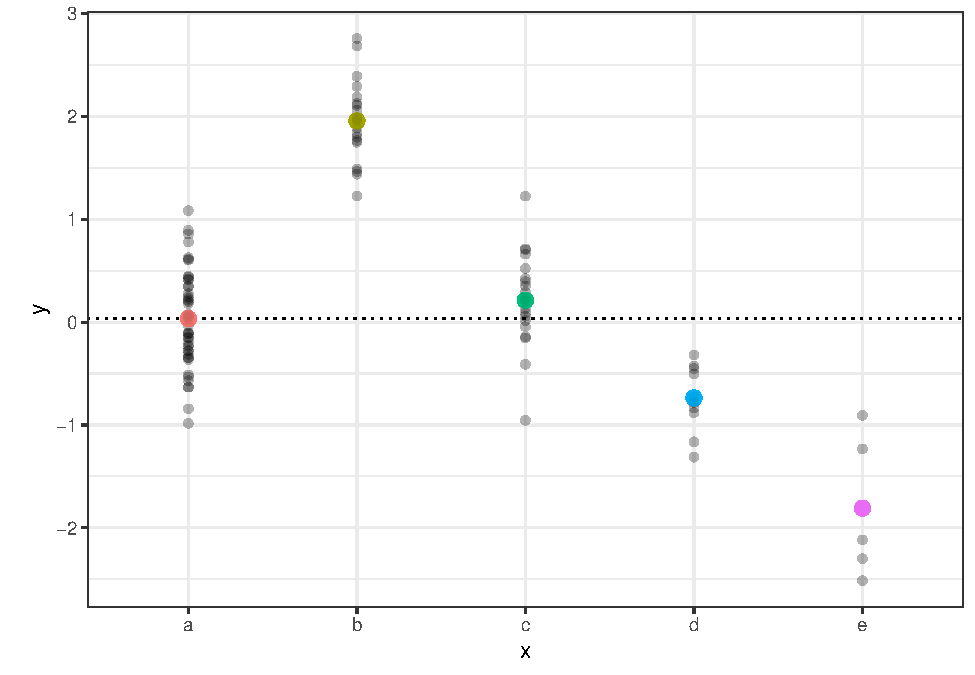
\includegraphics[width=3.5cm]{_bookdown_files/_main_files/figure-latex/lasso-lambda-1.pdf}
    \end{subfigure}
    \qquad
    \begin{subfigure}[b]{3cm}
      \centering
      \caption{$\lambda = 0.1$}
      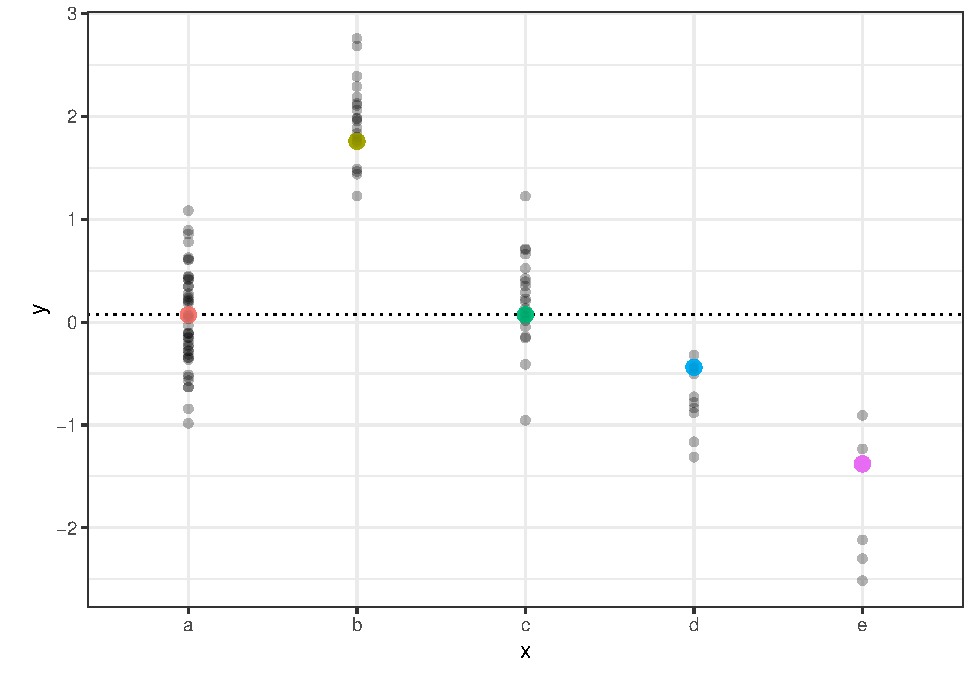
\includegraphics[width=3.5cm]{_bookdown_files/_main_files/figure-latex/lasso-lambda-2.pdf}
    \end{subfigure}
    \par\medskip
    \begin{subfigure}[b]{3cm}
      \centering
      \caption{$\lambda = 1$}
      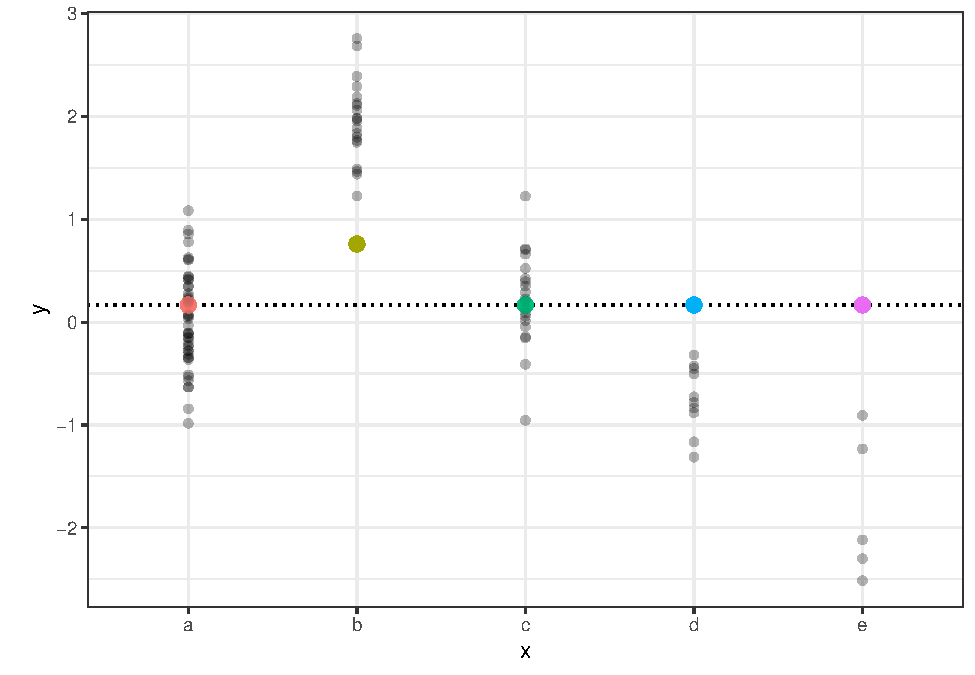
\includegraphics[width=3.5cm]{_bookdown_files/_main_files/figure-latex/lasso-lambda-3.pdf}
    \end{subfigure}
    \qquad
    \begin{subfigure}[b]{3cm}
      \centering
      \caption{$\lambda = 10$}
      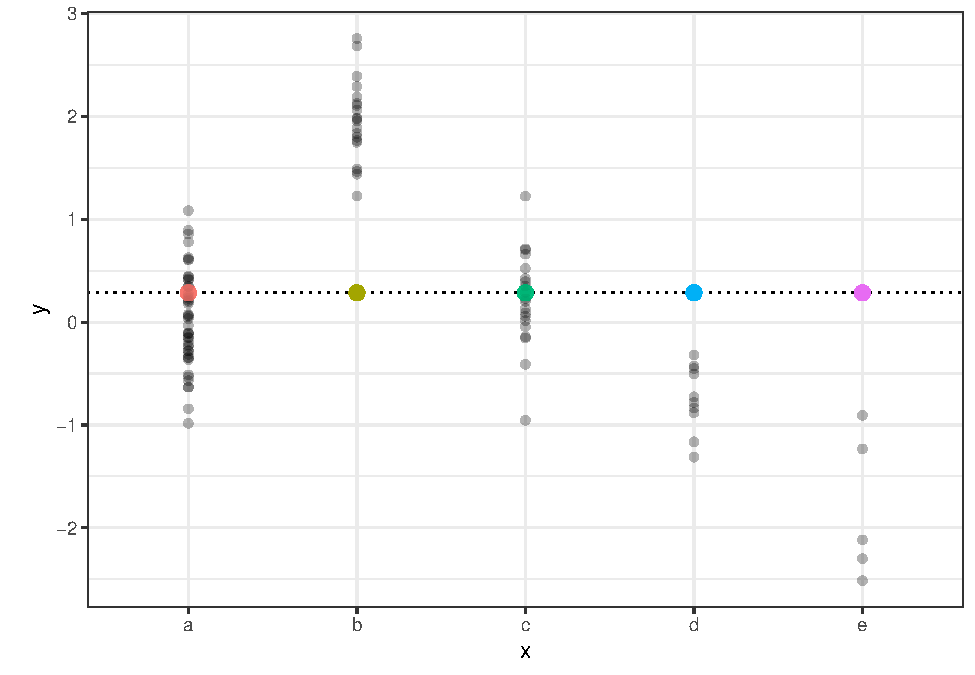
\includegraphics[width=3.5cm]{_bookdown_files/_main_files/figure-latex/lasso-lambda-4.pdf}
    \end{subfigure}
  \end{figure}
\end{column}
\begin{column}{0.45\linewidth}
  \begin{figure}
    \centering
    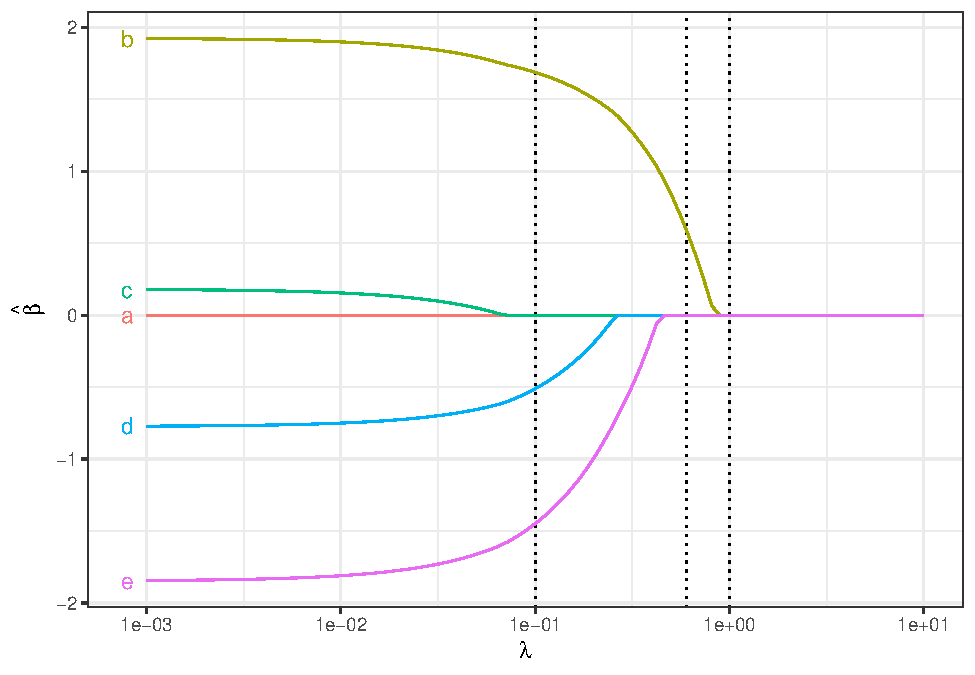
\includegraphics[width=5cm]{_bookdown_files/_main_files/figure-latex/lasso-lambda-5.pdf}
  \end{figure}
\end{column}
\end{columns}

\end{frame}

%%%%%%%%%%%%%%%%%%%%%%%%%%%%%%%%%%%%%%%%%%%%%%%%%%%%%%%%%%%%%
\begin{frame}
\frametitle{Elastic Net}

\fontsize{9pt}{11pt}\selectfont

\begin{columns}
\begin{column}{0.8\linewidth}
  \begin{block}{Stima di Massima Verosimiglianza con Penalizzazione}
    $$
    \hat{\boldsymbol{\beta}} = \argmin_{\boldsymbol{\beta}\in\mathbb{R}^{p+1}}{\left\{
    D(\boldsymbol{\beta}, \boldsymbol{y}) +
    \lambda 
    \sum_{j=1}^p{\left(\alpha |\beta_j| + (1 - \alpha) |\beta_j|^2\right)}
    \right\}}
    $$
    dove
    \begin{itemize}
      \item $\|\boldsymbol{\beta}_{\setminus0}\|_1 = \sum_{j=1}^p{|\beta_j|}$
      \item $\|\boldsymbol{\beta}_{\setminus0}\|_2^2 = \sum_{j=1}^p{\beta_j^2}$
      \item $\lambda\ge0$ iperparametro di penalizzazione
      \item $\alpha \in [0,1]$ iperparametro che determina il peso della LASSO
    \end{itemize}
    
    \vspace{0.2cm}
    
    Modello sottostante:GLM
  \end{block}
\end{column}
\end{columns}

\end{frame}



%%%%%%%%%%%%%%%%%%%%%%%%%%%%%%%%%%%%%%%%%%%%%%%%%%%%%%%%%%%%%
\subsection{Stimatori Bayesiani per i GLM}

%%%%%%%%%%%%%%%%%%%%%%%%%%%%%%%%%%%%%%%%%%%%%%%%%%%%%%%%%%%%%
\begin{frame}
\frametitle{Il Framework Bayesiano}

\begin{columns}

\begin{column}{0.3\linewidth}
  \begin{block}{Teorema di Bayes}
  $$
  \pi(\theta|\boldsymbol{y}) = \frac{p(\boldsymbol{y}|\theta)\pi(\theta)}{p(\boldsymbol{y})}
  $$
  \end{block}
\end{column}

\begin{column}{0.7\linewidth}
  \begin{figure}
      \centering
      \includegraphics[width=9cm]{_bookdown_files/_main_files/figure-latex/bayes-normal-1.pdf}
      \label{fig:bayes-normal}
    \end{figure}
\end{column}

\end{columns}


\end{frame}


%%%%%%%%%%%%%%%%%%%%%%%%%%%%%%%%%%%%%%%%%%%%%%%%%%%%%%%%%%%%%
\begin{frame}
\frametitle{Stimatori Bayesiani per i GLM}

\fontsize{9pt}{11pt}\selectfont

\begin{columns}[T]

\uncover<1->{
  \begin{column}{0.5\linewidth}
    \begin{block}{Stima di Massima Verosimiglianza}
      \begin{align*}
        \hat{\boldsymbol{\beta}}^{ML} & = \argmax_{\boldsymbol{\beta}\in\mathbb{R}^{p+1}}{L\left(\boldsymbol{\beta}, \phi \mid \boldsymbol{y}\right)} \\
        & = \argmax_{\boldsymbol{\beta}\in\mathbb{R}^{p+1}}{\ell\left(\boldsymbol{\beta}, \phi \mid \boldsymbol{y}\right)} \\
        & = \argmin_{\boldsymbol{\beta}\in\mathbb{R}^{p+1}}{D\left(\boldsymbol{\beta}, \boldsymbol{y}\right)} \\
      \end{align*}
    \end{block}
  \end{column}
}
\uncover<2->{
  \begin{column}{0.5\linewidth}
    \begin{block}{Stima di Massimo a Posteriori}
      \begin{align*}
        \hat{\boldsymbol{\beta}}^{MAP} & = \argmax_{\boldsymbol{\beta}\in\mathbb{R}^{p+1}}{\pi\left(\boldsymbol{\beta}, \phi \mid \boldsymbol{y}\right)} \\
        & = \argmax_{\boldsymbol{\beta}\in\mathbb{R}^{p+1}}{\left\{L\left(\boldsymbol{\beta}, \phi \mid \boldsymbol{y}\right) \pi(\boldsymbol{\beta}) \right\}} \\
        & = \argmax_{\boldsymbol{\beta}\in\mathbb{R}^{p+1}}{\left\{\ell\left(\boldsymbol{\beta}, \phi \mid \boldsymbol{y}\right) + \log{\left(\pi(\boldsymbol{\beta})\right)} \right\}} \\
        & = \argmin_{\boldsymbol{\beta}\in\mathbb{R}^{p+1}}{\left\{
          D(\boldsymbol{\beta}, \boldsymbol{y}) -2\phi \log{\left(\pi(\boldsymbol{\beta})\right)}           \right\}}
      \end{align*}
    \end{block}
  \end{column}
}

\end{columns}

\end{frame}



%%%%%%%%%%%%%%%%%%%%%%%%%%%%%%%%%%%%%%%%%%%%%%%%%%%%%%%%%%%%%
\begin{frame}
\frametitle{Regressione Ridge e LASSO come Stimatori Bayesiani}

\fontsize{9pt}{11pt}\selectfont

\begin{figure}
  % \captionsetup{justification=raggedleft}
  \centering
  \begin{subfigure}[b]{5cm}
    \captionsetup{justification=raggedright}
    \centering
    \caption{\hspace{0.9cm} Distribuzione Normale \\ \hspace{0.9cm} $\Rightarrow$ Regressione Ridge}
    \includegraphics[width=4cm]{_bookdown_files/_main_files/figure-latex/normal-laplace-1.pdf}
  \end{subfigure}
  \qquad
  \begin{subfigure}[b]{5cm}
    \captionsetup{justification=raggedright}
    \centering
    \caption{\hspace{0.9cm} Distribuzione di Laplace \\ \hspace{0.9cm} $\Rightarrow$ Regressione LASSO}
    \includegraphics[width=4cm]{_bookdown_files/_main_files/figure-latex/normal-laplace-2.pdf}
  \end{subfigure}
  % \qquad
  % \par\medskip
  \begin{subfigure}[b]{5cm}
  % \begin{subfigure}[b]{5.9cm}
    \captionsetup{justification=raggedright}
    \centering
    \caption{\hspace{0.9cm} Distribuzion intermedia \\ \hspace{0.9cm} $\Rightarrow$ Elastic Net}
    \includegraphics[width=4cm]{_bookdown_files/_main_files/figure-latex/normal-laplace-3.pdf}
  \end{subfigure}
\end{figure}

\end{frame}


%%%%%%%%%%%%%%%%%%%%%%%%%%%%%%%%%%%%%%%%%%%%%%%%%%%%%%%%%%%%%
\begin{frame}
\frametitle{Considerazioni sugli Stimatori Bayesiani}

\fontsize{9pt}{11pt}\selectfont

\begin{columns}[T]

\uncover<1->{
  \begin{column}{0.5\linewidth}
    \begin{block}{Altri distribuzioni a priori}
      \begin{itemize}
        \setlength\itemsep{0.2cm}
        \setlength\topsep{0.2cm}
        \item Diverse varianze a priori
          $$
          \beta_j\sim\mathcal{N}(0, \sigma_j^2)
          $$
        \item Diverse medie a priori
          $$
          \beta_j\sim\mathcal{N}(\beta_{j0}, \sigma_j^2)
          $$
        \item Altre distribuzioni a priori
          $$
          \pi(\beta_j) =
          \begin{cases}
            \frac{\sqrt{2}}{\sqrt{\pi}\sigma}e^{-\frac{1}{2\sigma^2}\beta_j^2} & \text{if } \beta_j \ge 0 \\
            0 & \text{altrimenti}
          \end{cases}
          $$
      \end{itemize}
    \end{block}
  \end{column}
}
\uncover<2->{
  \begin{column}{0.5\linewidth}
    \begin{block}{Vantaggi stimatori Bayesiani}
      \begin{itemize}
        \setlength\itemsep{0.2cm}
        % \setlength\topsep{0.2cm}
        \item Introduzione informazione esterna ai dati con una robusta metodologia statistica
        \item Rimpiazzamento degli offset \\
          Scelgo $\sigma_j^2$ tale che $\hat{\boldsymbol{\beta}}^{MAP} = \hat{\boldsymbol{\beta}}^{\textrm{offset}}$
          \begin{itemize}
            % \setlength\itemsep{0.1cm}
            % \setlength\topsep{1cm}
            \fontsize{9pt}{11pt}\selectfont
            \item[\faCaretRight] Ho accortezza di quanto è forte la correzzione applicata
            \item[\faCaretRight] Se cambio qualche altro parametro e rifitto il modello, in automatico $\hat{\boldsymbol{\beta}}^{MAP}$ viene ristimato
          \end{itemize}
      \end{itemize}
    \end{block}
  \end{column}
}

\end{columns}


\end{frame}


%%%%%%%%%%%%%%%%%%%%%%%%%%%%%%%%%%%%%%%%%%%%%%%%%%%%%%%%%%%%%
\subsection{Algoritmi di Machine Learning}

%%%%%%%%%%%%%%%%%%%%%%%%%%%%%%%%%%%%%%%%%%%%%%%%%%%%%%%%%%%%%
\begin{frame}
\frametitle{Algoritmi di Machine Learning}

\fontsize{9pt}{11pt}\selectfont

\begin{columns}[T]

\uncover<1->{
  \begin{column}{0.5\linewidth}
    \begin{block}{Modelli di Machine Learning}
      \begin{itemize}
        \item Gradient Boosting Machine (GBM)
        \item Random Forest (RF)
        \item Neural Network (NN)
        \item Altri \dots
      \end{itemize}
    \end{block}
  \end{column}
}
\uncover<2->{
  \begin{column}{0.5\linewidth}
    \begin{block}{Caratteristiche}
      \begin{itemize}
        \item Funzione di regressione con minime assunzioni
          $$E(Y_i) = \boldsymbol{f}(x_{i1}, \dots, x_{ip})$$
        \item Sofisticati algoritmi per prevenire l'overfitting
      \end{itemize}
    \end{block}
  \end{column}
}

\end{columns}

\end{frame}


%%%%%%%%%%%%%%%%%%%%%%%%%%%%%%%%%%%%%%%%%%%%%%%%%%%%%%%%%%%%%
\subsection{Confronto tra i modelli}

%%%%%%%%%%%%%%%%%%%%%%%%%%%%%%%%%%%%%%%%%%%%%%%%%%%%%%%%%%%%%
\begin{frame}
\frametitle{Confronto tra i modelli}

\fontsize{9pt}{11pt}\selectfont

\begin{columns}[T]

\uncover<1->{
  \begin{column}{0.5\linewidth}
    \begin{block}{GLM Classici vs GBM/RF/NN}
    % \begin{block}{GLM Classici vs GBM, RF e NN}
      \vspace{0.1cm}
      \begin{itemize}
        \setlength\itemsep{0.2cm}
        \item[\textcolor{ForestGreen}{\faThumbsOUp}] Maggior interpretabilità
        \item[\textcolor{ForestGreen}{\faThumbsOUp}] Maggior controllo delle variabili
          \begin{itemize}
            \fontsize{9pt}{11pt}\selectfont
            \item[\textcolor{ForestGreen}{\faCaretRight}] Selezione variabili
            \item[\textcolor{ForestGreen}{\faCaretRight}] Effetti variabili quantitative
            \item[\textcolor{ForestGreen}{\faCaretRight}] Offset
          \end{itemize}
        \item[\textcolor{ForestGreen}{\faThumbsOUp}] Facile utilizzo di informazioni esterne
        \item[\faThumbsODown] Minore automazione e scalabilità
        \item[\faThumbsODown] Minore flessibilità
      \end{itemize}
    \end{block}
  \end{column}
}
\uncover<2->{
  \begin{column}{0.5\linewidth}
    \begin{block}{GLM Advancements vs GLM Classici \vphantom{/}}
      \vspace{0.1cm}
      \begin{itemize}
        \setlength\itemsep{0.2cm}
        \item[\textcolor{ForestGreen}{\faThumbsOUp}] Mantenimento interpretabilità
        \item[\textcolor{ForestGreen}{\faThumbsOUp}] Mantenimento controllo delle variabili
        \item[\textcolor{ForestGreen}{\faThumbsOUp}] Miglior utilizzo delle informazioni esterne (stimatori bayesiani)
        \item[\textcolor{ForestGreen}{\faThumbsOUp}] Maggior automazione e scalabilità
          \begin{itemize}
            \fontsize{9pt}{11pt}\selectfont
            \item[\textcolor{ForestGreen}{\faCaretRight}] Selezione variabili
            \item[\textcolor{ForestGreen}{\faCaretRight}] Effetti variabili quantitative
          \end{itemize}
      \end{itemize}
    \end{block}
  \end{column}
}

\end{columns}

\end{frame}


%%%%%%%%%%%%%%%%%%%%%%%%%%%%%%%%%%%%%%%%%%%%%%%%%%%%%%%%%%%%%
\begin{frame}
\frametitle{L'importanza dell'attuario}

\end{frame}




%%%%%%%%%%%%%%%%%%%%%%%%%%%%%%%%%%%%%%%%%%%%%%%%%%%%%%%%%%%%%
\section{Applicazione Pratica}

\begin{frame}{Indice}
  \tableofcontents[currentsection]
\end{frame}


%%%%%%%%%%%%%%%%%%%%%%%%%%%%%%%%%%%%%%%%%%%%%%%%%%%%%%%%%%%%%
\begin{frame}
\frametitle{Esposizione e Variabile Risposta}

\fontsize{9pt}{11pt}\selectfont

\begin{table}[!h]
  \centering
  \begin{tabular}{lcccccc}
    \toprule
    \textbf{Set} & \textbf{Osservazioni} & \textbf{\makecell[c]{Esposizione\\(rischi anno)}} & \textbf{Assicurati} & \textbf{\makecell[c]{Esposizione per\\Assicurato}} & \textbf{\makecell[c]{Numero\\Sinistri}} & \textbf{\makecell[c]{Frequenza\\Sinistri}}\\
    \midrule[\heavyrulewidth]
    Train & 227 226 & 107 998.4 & 27 346 & 3.95 & 4 823 & 0.045\\
    Test  &  56 603 &  26 806.3 &  6 824 & 3.93 & 1 131 & 0.042\\
    \midrule
    Tot   & 283 829 & 134 804.7 & 34 170 & 3.95 & 5 954 & 0.044\\
    \bottomrule
  \end{tabular}
\end{table}

\end{frame}


%%%%%%%%%%%%%%%%%%%%%%%%%%%%%%%%%%%%%%%%%%%%%%%%%%%%%%%%%%%%%
\begin{frame}
\frametitle{Variabili esplicative}

\fontsize{9pt}{11pt}\selectfont

\begin{table}[!h]
  \centering
  \begin{tabular}{lc}
    \toprule
    \textbf{Descrizione} & \textbf{\makecell[c]{Numero di variabili\\per categoria}}\\
    \midrule[\heavyrulewidth]
    \cellcolor{gray!6}{Informazioni sul veicolo assicurato} & \cellcolor{gray!6}{12}\\
    Informazioni generiche sul contraente & 14\\
    \cellcolor{gray!6}{Informazioni assicurative sul contraente} & \cellcolor{gray!6}{9}\\
    Opzioni sulla polizza assicurativa & 11\\
    \cellcolor{gray!6}{Customer information on the policyholder} & \cellcolor{gray!6}{2}\\
    Dati telematici & 4\\
    \midrule
    \textbf{Totale} & \textbf{52}\\
    \bottomrule
  \end{tabular}
\end{table}

\end{frame}


%%%%%%%%%%%%%%%%%%%%%%%%%%%%%%%%%%%%%%%%%%%%%%%%%%%%%%%%%%%%%
\begin{frame}
\frametitle{Modelli e Valutazione}

\fontsize{9pt}{11pt}\selectfont

\begin{columns}[T]

\uncover<1->{
  \begin{column}{0.5\linewidth}
    \begin{block}{Modelli considerati}
      % \vspace{0.1cm}
      \begin{table}[!h]
        % \caption{\label{tab:models-list}List of models developed.}
        \centering
        \begin{tabular}[t]{ll}
          \toprule
          \textbf{Id} & \textbf{Model}\\
          \midrule[\heavyrulewidth]
          \cellcolor{gray!6}{Mod1} & \cellcolor{gray!6}{GLM Tot}\\
          Mod2 & Elastic Net Tot\\
          \cellcolor{gray!6}{Mod3} & \cellcolor{gray!6}{Ridge Tot}\\
          Mod4 & GLM AIC\\
          \cellcolor{gray!6}{Mod5} & \cellcolor{gray!6}{Elastic Net AIC}\\
          Mod6 & GAM AIC\\
          \cellcolor{gray!6}{Mod7} & \cellcolor{gray!6}{GBM Tot}\\
          \bottomrule
        \end{tabular}
      \end{table}
    \end{block}
  \end{column}
}
\uncover<2->{
  \begin{column}{0.5\linewidth}
    \begin{block}{Valutazione}
      \vspace{1cm}
      Devianza della distribuzione di Poisson calcolata sul test set
      $$
      D(\hat{\boldsymbol{\beta}}, \boldsymbol{y}) = 2\,\sum_{i=1}^{n}{\left\{ y_i \log{\left(\frac{y_i}{\hat{\mu}_i}\right)} - \left( y_i - \hat{\mu}_i \right) \right\}}
      $$
    \end{block}
  \end{column}
}

\end{columns}


\end{frame}


%%%%%%%%%%%%%%%%%%%%%%%%%%%%%%%%%%%%%%%%%%%%%%%%%%%%%%%%%%%%%
\begin{frame}
\frametitle{Titolo di prova capitolo 3}

\end{frame}



\end{document}
